\documentclass[twoside]{book}

% Packages required by doxygen
\usepackage{fixltx2e}
\usepackage{calc}
\usepackage{doxygen}
\usepackage[export]{adjustbox} % also loads graphicx
\usepackage{graphicx}
\usepackage[utf8]{inputenc}
\usepackage{makeidx}
\usepackage{multicol}
\usepackage{multirow}
\PassOptionsToPackage{warn}{textcomp}
\usepackage{textcomp}
\usepackage[nointegrals]{wasysym}
\usepackage[table]{xcolor}

% Font selection
\usepackage[T1]{fontenc}
\usepackage[scaled=.90]{helvet}
\usepackage{courier}
\usepackage{amssymb}
\usepackage{sectsty}
\renewcommand{\familydefault}{\sfdefault}
\allsectionsfont{%
  \fontseries{bc}\selectfont%
  \color{darkgray}%
}
\renewcommand{\DoxyLabelFont}{%
  \fontseries{bc}\selectfont%
  \color{darkgray}%
}
\newcommand{\+}{\discretionary{\mbox{\scriptsize$\hookleftarrow$}}{}{}}

% Page & text layout
\usepackage{geometry}
\geometry{%
  a4paper,%
  top=2.5cm,%
  bottom=2.5cm,%
  left=2.5cm,%
  right=2.5cm%
}
\tolerance=750
\hfuzz=15pt
\hbadness=750
\setlength{\emergencystretch}{15pt}
\setlength{\parindent}{0cm}
\setlength{\parskip}{3ex plus 2ex minus 2ex}
\makeatletter
\renewcommand{\paragraph}{%
  \@startsection{paragraph}{4}{0ex}{-1.0ex}{1.0ex}{%
    \normalfont\normalsize\bfseries\SS@parafont%
  }%
}
\renewcommand{\subparagraph}{%
  \@startsection{subparagraph}{5}{0ex}{-1.0ex}{1.0ex}{%
    \normalfont\normalsize\bfseries\SS@subparafont%
  }%
}
\makeatother

% Headers & footers
\usepackage{fancyhdr}
\pagestyle{fancyplain}
\fancyhead[LE]{\fancyplain{}{\bfseries\thepage}}
\fancyhead[CE]{\fancyplain{}{}}
\fancyhead[RE]{\fancyplain{}{\bfseries\leftmark}}
\fancyhead[LO]{\fancyplain{}{\bfseries\rightmark}}
\fancyhead[CO]{\fancyplain{}{}}
\fancyhead[RO]{\fancyplain{}{\bfseries\thepage}}
\fancyfoot[LE]{\fancyplain{}{}}
\fancyfoot[CE]{\fancyplain{}{}}
\fancyfoot[RE]{\fancyplain{}{\bfseries\scriptsize Generated by Doxygen }}
\fancyfoot[LO]{\fancyplain{}{\bfseries\scriptsize Generated by Doxygen }}
\fancyfoot[CO]{\fancyplain{}{}}
\fancyfoot[RO]{\fancyplain{}{}}
\renewcommand{\footrulewidth}{0.4pt}
\renewcommand{\chaptermark}[1]{%
  \markboth{#1}{}%
}
\renewcommand{\sectionmark}[1]{%
  \markright{\thesection\ #1}%
}

% Indices & bibliography
\usepackage{natbib}
\usepackage[titles]{tocloft}
\setcounter{tocdepth}{3}
\setcounter{secnumdepth}{5}
\makeindex

% Hyperlinks (required, but should be loaded last)
\usepackage{ifpdf}
\ifpdf
  \usepackage[pdftex,pagebackref=true]{hyperref}
\else
  \usepackage[ps2pdf,pagebackref=true]{hyperref}
\fi
\hypersetup{%
  colorlinks=true,%
  linkcolor=blue,%
  citecolor=blue,%
  unicode%
}

% Custom commands
\newcommand{\clearemptydoublepage}{%
  \newpage{\pagestyle{empty}\cleardoublepage}%
}

\usepackage{caption}
\captionsetup{labelsep=space,justification=centering,font={bf},singlelinecheck=off,skip=4pt,position=top}

%===== C O N T E N T S =====

\begin{document}

% Titlepage & ToC
\hypersetup{pageanchor=false,
             bookmarksnumbered=true,
             pdfencoding=unicode
            }
\pagenumbering{alph}
\begin{titlepage}
\vspace*{7cm}
\begin{center}%
{\Large T\+M\+AP }\\
\vspace*{1cm}
{\large Generated by Doxygen 1.8.13}\\
\end{center}
\end{titlepage}
\clearemptydoublepage
\pagenumbering{roman}
\tableofcontents
\clearemptydoublepage
\pagenumbering{arabic}
\hypersetup{pageanchor=true}

%--- Begin generated contents ---
\chapter{Hierarchical Index}
\section{Class Hierarchy}
This inheritance list is sorted roughly, but not completely, alphabetically\+:\begin{DoxyCompactList}
\item \contentsline{section}{tmap\+:\+:Graph\+Properties}{\pageref{structtmap_1_1GraphProperties}}{}
\item \contentsline{section}{tmap\+:\+:Layout\+Configuration}{\pageref{structtmap_1_1LayoutConfiguration}}{}
\item \contentsline{section}{tmap\+:\+:L\+S\+H\+Forest}{\pageref{classtmap_1_1LSHForest}}{}
\item \contentsline{section}{tmap\+:\+:Map\+Key\+Pointer}{\pageref{structtmap_1_1MapKeyPointer}}{}
\item \contentsline{section}{tmap\+:\+:Minhash}{\pageref{classtmap_1_1Minhash}}{}
\begin{DoxyCompactList}
\item \contentsline{section}{Py\+Minhash}{\pageref{classPyMinhash}}{}
\end{DoxyCompactList}
\item \contentsline{section}{tmap\+:\+:Simple\+Hash}{\pageref{structtmap_1_1SimpleHash}}{}
\item \contentsline{section}{tmap\+:\+:Timer}{\pageref{classtmap_1_1Timer}}{}
\end{DoxyCompactList}

\chapter{Class Index}
\section{Class List}
Here are the classes, structs, unions and interfaces with brief descriptions\+:\begin{DoxyCompactList}
\item\contentsline{section}{\hyperlink{structGraphProperties}{Graph\+Properties} \\*The properties of a generated graph. An instance of this struct is returned from the layout functions }{\pageref{structGraphProperties}}{}
\item\contentsline{section}{\hyperlink{structLayoutConfiguration}{Layout\+Configuration} \\*A struct containing all the configuration options available for and applied to a layout }{\pageref{structLayoutConfiguration}}{}
\item\contentsline{section}{\hyperlink{classLSHForest}{L\+S\+H\+Forest} \\*Provides locality sensitive hashing forest functionalities }{\pageref{classLSHForest}}{}
\item\contentsline{section}{\hyperlink{structMapKeyPointer}{Map\+Key\+Pointer} \\*The pointer map used for pointing to the keys from the sorted hash map }{\pageref{structMapKeyPointer}}{}
\item\contentsline{section}{\hyperlink{classMinhash}{Minhash} \\*An implementation of Min\+Hash and weighted Min\+Hash using S\+H\+A1 }{\pageref{classMinhash}}{}
\item\contentsline{section}{\hyperlink{classsha1_1_1SHA1}{sha1\+::\+S\+H\+A1} }{\pageref{classsha1_1_1SHA1}}{}
\item\contentsline{section}{\hyperlink{structSimpleHash}{Simple\+Hash} \\*Hash struct used for the sparsepp sparse hash map }{\pageref{structSimpleHash}}{}
\item\contentsline{section}{\hyperlink{classTimer}{Timer} \\*A simple timer class used to check performance during development }{\pageref{classTimer}}{}
\end{DoxyCompactList}

\chapter{File Index}
\section{File List}
Here is a list of all documented files with brief descriptions\+:\begin{DoxyCompactList}
\item\contentsline{section}{src/tmap/\hyperlink{bindings_8cc}{bindings.\+cc} \\*Pybind11 bindings for tmap }{\pageref{bindings_8cc}}{}
\item\contentsline{section}{src/tmap/\hyperlink{layout_8cc}{layout.\+cc} \\*Functions used for generating graph layouts from \hyperlink{classLSHForest}{L\+S\+H\+Forest} instances and edge lists }{\pageref{layout_8cc}}{}
\item\contentsline{section}{src/tmap/\hyperlink{layout_8hh}{layout.\+hh} \\*Functions used for generating graph layouts from \hyperlink{classLSHForest}{L\+S\+H\+Forest} instances and edge lists }{\pageref{layout_8hh}}{}
\item\contentsline{section}{src/tmap/\hyperlink{lshforest_8cc}{lshforest.\+cc} \\*An L\+SH forest algorithm implementation }{\pageref{lshforest_8cc}}{}
\item\contentsline{section}{src/tmap/\hyperlink{lshforest_8hh}{lshforest.\+hh} \\*An L\+SH forest algorithm implementation }{\pageref{lshforest_8hh}}{}
\item\contentsline{section}{src/tmap/\hyperlink{minhash_8cc}{minhash.\+cc} \\*A Min\+Hash algorithm implementation }{\pageref{minhash_8cc}}{}
\item\contentsline{section}{src/tmap/\hyperlink{minhash_8hh}{minhash.\+hh} \\*A Min\+Hash algorithm implementation }{\pageref{minhash_8hh}}{}
\item\contentsline{section}{src/tmap/{\bfseries Tiny\+S\+H\+A1.\+hh} }{\pageref{TinySHA1_8hh}}{}
\end{DoxyCompactList}

\chapter{Class Documentation}
\hypertarget{structtmap_1_1GraphProperties}{}\section{tmap\+:\+:Graph\+Properties Struct Reference}
\label{structtmap_1_1GraphProperties}\index{tmap\+::\+Graph\+Properties@{tmap\+::\+Graph\+Properties}}


The properties of a generated graph. An instance of this struct is returned from the layout functions.  




{\ttfamily \#include $<$layout.\+hh$>$}

\subsection*{Public Attributes}
\begin{DoxyCompactItemize}
\item 
\mbox{\Hypertarget{structtmap_1_1GraphProperties_a51fa52c1cc9c8d382d507349e99447be}\label{structtmap_1_1GraphProperties_a51fa52c1cc9c8d382d507349e99447be}} 
float \hyperlink{structtmap_1_1GraphProperties_a51fa52c1cc9c8d382d507349e99447be}{mst\+\_\+weight} = 0.\+0
\begin{DoxyCompactList}\small\item\em The total weight of the created spanning tree. \end{DoxyCompactList}\item 
\mbox{\Hypertarget{structtmap_1_1GraphProperties_a3467571c1e645268e55416504809f7c5}\label{structtmap_1_1GraphProperties_a3467571c1e645268e55416504809f7c5}} 
uint32\+\_\+t \hyperlink{structtmap_1_1GraphProperties_a3467571c1e645268e55416504809f7c5}{n\+\_\+connected\+\_\+components} = 0
\begin{DoxyCompactList}\small\item\em The number of connected components. \end{DoxyCompactList}\item 
\mbox{\Hypertarget{structtmap_1_1GraphProperties_a954e8fd087b44b3c568ea07ae2f1efea}\label{structtmap_1_1GraphProperties_a954e8fd087b44b3c568ea07ae2f1efea}} 
uint32\+\_\+t \hyperlink{structtmap_1_1GraphProperties_a954e8fd087b44b3c568ea07ae2f1efea}{n\+\_\+isolated\+\_\+vertices} = 0
\begin{DoxyCompactList}\small\item\em The number of isolated (lone) vertices. \end{DoxyCompactList}\item 
\mbox{\Hypertarget{structtmap_1_1GraphProperties_af4c85653b3bf56c6dbf19d7a38af40bc}\label{structtmap_1_1GraphProperties_af4c85653b3bf56c6dbf19d7a38af40bc}} 
std\+::vector$<$ uint32\+\_\+t $>$ \hyperlink{structtmap_1_1GraphProperties_af4c85653b3bf56c6dbf19d7a38af40bc}{degrees}
\begin{DoxyCompactList}\small\item\em The degrees of the vertices in the graph. \end{DoxyCompactList}\item 
\mbox{\Hypertarget{structtmap_1_1GraphProperties_a04c11168f810fdaf8b7bfecf96413ba7}\label{structtmap_1_1GraphProperties_a04c11168f810fdaf8b7bfecf96413ba7}} 
std\+::vector$<$ std\+::vector$<$ uint32\+\_\+t $>$ $>$ \hyperlink{structtmap_1_1GraphProperties_a04c11168f810fdaf8b7bfecf96413ba7}{adjacency\+\_\+list}
\begin{DoxyCompactList}\small\item\em The adjacency list of the spanning tree. \end{DoxyCompactList}\end{DoxyCompactItemize}


\subsection{Detailed Description}
The properties of a generated graph. An instance of this struct is returned from the layout functions. 

The documentation for this struct was generated from the following file\+:\begin{DoxyCompactItemize}
\item 
src/tmap/\hyperlink{layout_8hh}{layout.\+hh}\end{DoxyCompactItemize}

\hypertarget{structtmap_1_1LayoutConfiguration}{}\section{tmap\+:\+:Layout\+Configuration Struct Reference}
\label{structtmap_1_1LayoutConfiguration}\index{tmap\+::\+Layout\+Configuration@{tmap\+::\+Layout\+Configuration}}


A struct containing all the configuration options available for and applied to a layout.  




{\ttfamily \#include $<$layout.\+hh$>$}

\subsection*{Public Member Functions}
\begin{DoxyCompactItemize}
\item 
\mbox{\Hypertarget{structtmap_1_1LayoutConfiguration_a45335a69efe4408b49283554a3bb8875}\label{structtmap_1_1LayoutConfiguration_a45335a69efe4408b49283554a3bb8875}} 
\hyperlink{structtmap_1_1LayoutConfiguration_a45335a69efe4408b49283554a3bb8875}{Layout\+Configuration} ()
\begin{DoxyCompactList}\small\item\em Construct a new Layout Configuration object. \end{DoxyCompactList}\item 
std\+::string \hyperlink{structtmap_1_1LayoutConfiguration_a498341508ea4806795f44e376af18e11}{To\+String} () const
\begin{DoxyCompactList}\small\item\em Returns a string describing the set options. \end{DoxyCompactList}\end{DoxyCompactItemize}
\subsection*{Public Attributes}
\begin{DoxyCompactItemize}
\item 
int \hyperlink{structtmap_1_1LayoutConfiguration_a80ddc818732d708764fbd83ad7b7d153}{k}
\item 
int \hyperlink{structtmap_1_1LayoutConfiguration_ae63c0a1d5956cbdb837f3aff1978f867}{kc}
\item 
int \hyperlink{structtmap_1_1LayoutConfiguration_aa0b26a532aedb8f0fe4490c9c90b0e84}{fme\+\_\+iterations}
\item 
\mbox{\Hypertarget{structtmap_1_1LayoutConfiguration_a821bf612fb3063344ca0c6b161424a7b}\label{structtmap_1_1LayoutConfiguration_a821bf612fb3063344ca0c6b161424a7b}} 
bool \hyperlink{structtmap_1_1LayoutConfiguration_a821bf612fb3063344ca0c6b161424a7b}{fme\+\_\+randomize}
\begin{DoxyCompactList}\small\item\em Whether or not to randomize the layout at the start. \end{DoxyCompactList}\item 
\mbox{\Hypertarget{structtmap_1_1LayoutConfiguration_a7630a7d7513c3f51ea00802a3f67ba92}\label{structtmap_1_1LayoutConfiguration_a7630a7d7513c3f51ea00802a3f67ba92}} 
int \hyperlink{structtmap_1_1LayoutConfiguration_a7630a7d7513c3f51ea00802a3f67ba92}{fme\+\_\+threads}
\begin{DoxyCompactList}\small\item\em The number of threads for the fast multipole embedder. \end{DoxyCompactList}\item 
\mbox{\Hypertarget{structtmap_1_1LayoutConfiguration_a9e4d43d8f65c21404cc9912c11a3eba7}\label{structtmap_1_1LayoutConfiguration_a9e4d43d8f65c21404cc9912c11a3eba7}} 
int \hyperlink{structtmap_1_1LayoutConfiguration_a9e4d43d8f65c21404cc9912c11a3eba7}{fme\+\_\+precision}
\begin{DoxyCompactList}\small\item\em The number of coefficients of the multipole expansion. \end{DoxyCompactList}\item 
\mbox{\Hypertarget{structtmap_1_1LayoutConfiguration_adf81cfbcba521fd87a73dd25eb9c21e7}\label{structtmap_1_1LayoutConfiguration_adf81cfbcba521fd87a73dd25eb9c21e7}} 
int \hyperlink{structtmap_1_1LayoutConfiguration_adf81cfbcba521fd87a73dd25eb9c21e7}{sl\+\_\+repeats}
\begin{DoxyCompactList}\small\item\em The number of repeats of the scaling layout algorithm. \end{DoxyCompactList}\item 
\mbox{\Hypertarget{structtmap_1_1LayoutConfiguration_aefd713cfba563ea8ee9a432c0359c440}\label{structtmap_1_1LayoutConfiguration_aefd713cfba563ea8ee9a432c0359c440}} 
int \hyperlink{structtmap_1_1LayoutConfiguration_aefd713cfba563ea8ee9a432c0359c440}{sl\+\_\+extra\+\_\+scaling\+\_\+steps}
\begin{DoxyCompactList}\small\item\em Sets the number of repeats of the scaling. \end{DoxyCompactList}\item 
\mbox{\Hypertarget{structtmap_1_1LayoutConfiguration_af2e01075c5fe2a36c6018b40a6919d7a}\label{structtmap_1_1LayoutConfiguration_af2e01075c5fe2a36c6018b40a6919d7a}} 
double \hyperlink{structtmap_1_1LayoutConfiguration_af2e01075c5fe2a36c6018b40a6919d7a}{sl\+\_\+scaling\+\_\+min}
\begin{DoxyCompactList}\small\item\em The minimum scaling factor. \end{DoxyCompactList}\item 
\mbox{\Hypertarget{structtmap_1_1LayoutConfiguration_aa29669e99b7e1df2bcb95d6379da7cc3}\label{structtmap_1_1LayoutConfiguration_aa29669e99b7e1df2bcb95d6379da7cc3}} 
double \hyperlink{structtmap_1_1LayoutConfiguration_aa29669e99b7e1df2bcb95d6379da7cc3}{sl\+\_\+scaling\+\_\+max}
\begin{DoxyCompactList}\small\item\em The maximum scaling factor. \end{DoxyCompactList}\item 
\mbox{\Hypertarget{structtmap_1_1LayoutConfiguration_a618d286e035eca76e0e464513624beec}\label{structtmap_1_1LayoutConfiguration_a618d286e035eca76e0e464513624beec}} 
\hyperlink{layout_8hh_a50ec215c9e54cf12b9dd0a0056160761}{Scaling\+Type} \hyperlink{structtmap_1_1LayoutConfiguration_a618d286e035eca76e0e464513624beec}{sl\+\_\+scaling\+\_\+type}
\begin{DoxyCompactList}\small\item\em Defines the (relative) scale of the graph. \end{DoxyCompactList}\item 
\mbox{\Hypertarget{structtmap_1_1LayoutConfiguration_aff2347eb71c98bbc72f16b4de32d4af0}\label{structtmap_1_1LayoutConfiguration_aff2347eb71c98bbc72f16b4de32d4af0}} 
int \hyperlink{structtmap_1_1LayoutConfiguration_aff2347eb71c98bbc72f16b4de32d4af0}{mmm\+\_\+repeats}
\begin{DoxyCompactList}\small\item\em Number of repeats of the per-\/level layout algorithm. \end{DoxyCompactList}\item 
\hyperlink{layout_8hh_afdc98947e81dc6f4c30f256e6f42f90b}{Placer} \hyperlink{structtmap_1_1LayoutConfiguration_ae81108ee33f42b2c084b540f902bbb7d}{placer}
\item 
\hyperlink{layout_8hh_a8c7bb9956a1a724233182a166cfdc0ff}{Merger} \hyperlink{structtmap_1_1LayoutConfiguration_aeee45308fd8dbda38fbc7b8c7ff9212f}{merger}
\item 
double \hyperlink{structtmap_1_1LayoutConfiguration_a72fe4f8f738d2d400f70db97c4273a46}{merger\+\_\+factor}
\item 
int \hyperlink{structtmap_1_1LayoutConfiguration_a16109420c8ec0a4c3021345fd943daf6}{merger\+\_\+adjustment}
\item 
float \hyperlink{structtmap_1_1LayoutConfiguration_a9a97e2c0c9edb212190d3afcc3ce2924}{node\+\_\+size}
\end{DoxyCompactItemize}


\subsection{Detailed Description}
A struct containing all the configuration options available for and applied to a layout. 

\subsection{Member Function Documentation}
\mbox{\Hypertarget{structtmap_1_1LayoutConfiguration_a498341508ea4806795f44e376af18e11}\label{structtmap_1_1LayoutConfiguration_a498341508ea4806795f44e376af18e11}} 
\index{tmap\+::\+Layout\+Configuration@{tmap\+::\+Layout\+Configuration}!To\+String@{To\+String}}
\index{To\+String@{To\+String}!tmap\+::\+Layout\+Configuration@{tmap\+::\+Layout\+Configuration}}
\subsubsection{\texorpdfstring{To\+String()}{ToString()}}
{\footnotesize\ttfamily std\+::string tmap\+::\+Layout\+Configuration\+::\+To\+String (\begin{DoxyParamCaption}{ }\end{DoxyParamCaption}) const\hspace{0.3cm}{\ttfamily [inline]}}



Returns a string describing the set options. 

\begin{DoxyReturn}{Returns}
std\+::string 
\end{DoxyReturn}


\subsection{Member Data Documentation}
\mbox{\Hypertarget{structtmap_1_1LayoutConfiguration_aa0b26a532aedb8f0fe4490c9c90b0e84}\label{structtmap_1_1LayoutConfiguration_aa0b26a532aedb8f0fe4490c9c90b0e84}} 
\index{tmap\+::\+Layout\+Configuration@{tmap\+::\+Layout\+Configuration}!fme\+\_\+iterations@{fme\+\_\+iterations}}
\index{fme\+\_\+iterations@{fme\+\_\+iterations}!tmap\+::\+Layout\+Configuration@{tmap\+::\+Layout\+Configuration}}
\subsubsection{\texorpdfstring{fme\+\_\+iterations}{fme\_iterations}}
{\footnotesize\ttfamily int tmap\+::\+Layout\+Configuration\+::fme\+\_\+iterations}

Maximum number of iterations of the fast multipole embedder. \mbox{\Hypertarget{structtmap_1_1LayoutConfiguration_a80ddc818732d708764fbd83ad7b7d153}\label{structtmap_1_1LayoutConfiguration_a80ddc818732d708764fbd83ad7b7d153}} 
\index{tmap\+::\+Layout\+Configuration@{tmap\+::\+Layout\+Configuration}!k@{k}}
\index{k@{k}!tmap\+::\+Layout\+Configuration@{tmap\+::\+Layout\+Configuration}}
\subsubsection{\texorpdfstring{k}{k}}
{\footnotesize\ttfamily int tmap\+::\+Layout\+Configuration\+::k}

The number of nearest neighbors used to create the k-\/nearest neighbor graph. \mbox{\Hypertarget{structtmap_1_1LayoutConfiguration_ae63c0a1d5956cbdb837f3aff1978f867}\label{structtmap_1_1LayoutConfiguration_ae63c0a1d5956cbdb837f3aff1978f867}} 
\index{tmap\+::\+Layout\+Configuration@{tmap\+::\+Layout\+Configuration}!kc@{kc}}
\index{kc@{kc}!tmap\+::\+Layout\+Configuration@{tmap\+::\+Layout\+Configuration}}
\subsubsection{\texorpdfstring{kc}{kc}}
{\footnotesize\ttfamily int tmap\+::\+Layout\+Configuration\+::kc}

The scalar by which k is multiplied before querying the L\+SH forest. The results are then ordered decreasing based on linear-\/scan distances and the top k results returned. \mbox{\Hypertarget{structtmap_1_1LayoutConfiguration_aeee45308fd8dbda38fbc7b8c7ff9212f}\label{structtmap_1_1LayoutConfiguration_aeee45308fd8dbda38fbc7b8c7ff9212f}} 
\index{tmap\+::\+Layout\+Configuration@{tmap\+::\+Layout\+Configuration}!merger@{merger}}
\index{merger@{merger}!tmap\+::\+Layout\+Configuration@{tmap\+::\+Layout\+Configuration}}
\subsubsection{\texorpdfstring{merger}{merger}}
{\footnotesize\ttfamily \hyperlink{layout_8hh_a8c7bb9956a1a724233182a166cfdc0ff}{Merger} tmap\+::\+Layout\+Configuration\+::merger}

The vertex merging strategy applied during the coarsening phaseof the multilevel algorithm. \mbox{\Hypertarget{structtmap_1_1LayoutConfiguration_a16109420c8ec0a4c3021345fd943daf6}\label{structtmap_1_1LayoutConfiguration_a16109420c8ec0a4c3021345fd943daf6}} 
\index{tmap\+::\+Layout\+Configuration@{tmap\+::\+Layout\+Configuration}!merger\+\_\+adjustment@{merger\+\_\+adjustment}}
\index{merger\+\_\+adjustment@{merger\+\_\+adjustment}!tmap\+::\+Layout\+Configuration@{tmap\+::\+Layout\+Configuration}}
\subsubsection{\texorpdfstring{merger\+\_\+adjustment}{merger\_adjustment}}
{\footnotesize\ttfamily int tmap\+::\+Layout\+Configuration\+::merger\+\_\+adjustment}

The edge length adjustment of the merging algorithm. Does notapply to all merging strategies. \mbox{\Hypertarget{structtmap_1_1LayoutConfiguration_a72fe4f8f738d2d400f70db97c4273a46}\label{structtmap_1_1LayoutConfiguration_a72fe4f8f738d2d400f70db97c4273a46}} 
\index{tmap\+::\+Layout\+Configuration@{tmap\+::\+Layout\+Configuration}!merger\+\_\+factor@{merger\+\_\+factor}}
\index{merger\+\_\+factor@{merger\+\_\+factor}!tmap\+::\+Layout\+Configuration@{tmap\+::\+Layout\+Configuration}}
\subsubsection{\texorpdfstring{merger\+\_\+factor}{merger\_factor}}
{\footnotesize\ttfamily double tmap\+::\+Layout\+Configuration\+::merger\+\_\+factor}

The ratio of the sizes between two levels up to which the mergingis run. Does not apply to all merging strategies. \mbox{\Hypertarget{structtmap_1_1LayoutConfiguration_a9a97e2c0c9edb212190d3afcc3ce2924}\label{structtmap_1_1LayoutConfiguration_a9a97e2c0c9edb212190d3afcc3ce2924}} 
\index{tmap\+::\+Layout\+Configuration@{tmap\+::\+Layout\+Configuration}!node\+\_\+size@{node\+\_\+size}}
\index{node\+\_\+size@{node\+\_\+size}!tmap\+::\+Layout\+Configuration@{tmap\+::\+Layout\+Configuration}}
\subsubsection{\texorpdfstring{node\+\_\+size}{node\_size}}
{\footnotesize\ttfamily float tmap\+::\+Layout\+Configuration\+::node\+\_\+size}

The size of the nodes, which affects the magnitude of their repellingforce. Decreasing this value generally resolves overlaps in a verycrowded tree. \mbox{\Hypertarget{structtmap_1_1LayoutConfiguration_ae81108ee33f42b2c084b540f902bbb7d}\label{structtmap_1_1LayoutConfiguration_ae81108ee33f42b2c084b540f902bbb7d}} 
\index{tmap\+::\+Layout\+Configuration@{tmap\+::\+Layout\+Configuration}!placer@{placer}}
\index{placer@{placer}!tmap\+::\+Layout\+Configuration@{tmap\+::\+Layout\+Configuration}}
\subsubsection{\texorpdfstring{placer}{placer}}
{\footnotesize\ttfamily \hyperlink{layout_8hh_afdc98947e81dc6f4c30f256e6f42f90b}{Placer} tmap\+::\+Layout\+Configuration\+::placer}

The method by which the initial positons of the vertices at eachlevel are defined. 

The documentation for this struct was generated from the following file\+:\begin{DoxyCompactItemize}
\item 
tmap/\hyperlink{layout_8hh}{layout.\+hh}\end{DoxyCompactItemize}

\hypertarget{classtmap_1_1LSHForest}{}\section{tmap\+:\+:L\+S\+H\+Forest Class Reference}
\label{classtmap_1_1LSHForest}\index{tmap\+::\+L\+S\+H\+Forest@{tmap\+::\+L\+S\+H\+Forest}}


Provides locality sensitive hashing forest functionalities.  




{\ttfamily \#include $<$lshforest.\+hh$>$}

\subsection*{Public Member Functions}
\begin{DoxyCompactItemize}
\item 
\hyperlink{classtmap_1_1LSHForest_a153cb1f5090432257a17f2e9dacc32a0}{L\+S\+H\+Forest} (unsigned int d=128, unsigned int l=8, bool store=true, bool file\+\_\+backed=false)
\begin{DoxyCompactList}\small\item\em Construct a new \hyperlink{classtmap_1_1LSHForest}{L\+S\+H\+Forest} object. \end{DoxyCompactList}\item 
\mbox{\Hypertarget{classtmap_1_1LSHForest_a3ab5789f702f9dac3f801c7b9d53afd4}\label{classtmap_1_1LSHForest_a3ab5789f702f9dac3f801c7b9d53afd4}} 
\hyperlink{classtmap_1_1LSHForest_a3ab5789f702f9dac3f801c7b9d53afd4}{$\sim$\+L\+S\+H\+Forest} ()
\begin{DoxyCompactList}\small\item\em Destroy the \hyperlink{classtmap_1_1LSHForest}{L\+S\+H\+Forest} object. \end{DoxyCompactList}\item 
void \hyperlink{classtmap_1_1LSHForest_a480d0de16bc1e4b1365bf97b9b60223a}{Add} (std\+::vector$<$ uint32\+\_\+t $>$ \&vec)
\begin{DoxyCompactList}\small\item\em Add a Min\+Hash to this \hyperlink{classtmap_1_1LSHForest}{L\+S\+H\+Forest} instance. \end{DoxyCompactList}\item 
void \hyperlink{classtmap_1_1LSHForest_ab3f73f59918a37b63662679461828cbb}{Batch\+Add} (std\+::vector$<$ std\+::vector$<$ uint32\+\_\+t $>$$>$ \&vecs)
\begin{DoxyCompactList}\small\item\em Add Minhashes to this \hyperlink{classtmap_1_1LSHForest}{L\+S\+H\+Forest} (parallelized). \end{DoxyCompactList}\item 
\mbox{\Hypertarget{classtmap_1_1LSHForest_aba68c9cab8cc3c32e684e08b4f9d0a33}\label{classtmap_1_1LSHForest_aba68c9cab8cc3c32e684e08b4f9d0a33}} 
void \hyperlink{classtmap_1_1LSHForest_aba68c9cab8cc3c32e684e08b4f9d0a33}{Index} ()
\begin{DoxyCompactList}\small\item\em Create the index (trees). \end{DoxyCompactList}\item 
bool \hyperlink{classtmap_1_1LSHForest_a7785c1a7f17eddd5e943db4b5d6d7cf2}{Is\+Clean} ()
\begin{DoxyCompactList}\small\item\em Check whether the added Min\+Hashes have been indexed. \end{DoxyCompactList}\item 
void \hyperlink{classtmap_1_1LSHForest_a1731bf94cd09e7ebc4a10dd42145dc51}{Store} (const std\+::string \&path)
\begin{DoxyCompactList}\small\item\em Write / serialize the current L\+SH forest to the disk. \end{DoxyCompactList}\item 
void \hyperlink{classtmap_1_1LSHForest_a869273bd3d4c72c4c296dc42519558c8}{Restore} (const std\+::string \&path)
\begin{DoxyCompactList}\small\item\em Read / deserialize a L\+SH forest instance form the disk. The forest is indexed automatically. \end{DoxyCompactList}\item 
std\+::vector$<$ uint32\+\_\+t $>$ \hyperlink{classtmap_1_1LSHForest_a78106dd9e3a9a9ec012e5405445be78c}{Get\+Hash} (uint32\+\_\+t id)
\begin{DoxyCompactList}\small\item\em Get the Min\+Hash of an entry at a given index. The index is defined by order of insertion. \end{DoxyCompactList}\item 
void \hyperlink{classtmap_1_1LSHForest_a11ccbeea4356cce12b579566925d865f}{Get\+K\+N\+N\+Graph} (std\+::vector$<$ uint32\+\_\+t $>$ \&from, std\+::vector$<$ uint32\+\_\+t $>$ \&to, std\+::vector$<$ float $>$ \&weight, unsigned int k, unsigned int kc=10, bool weighted=false)
\begin{DoxyCompactList}\small\item\em Get the k-\/nearest neighbor graph of the data stored in this L\+SH forest instance. It will be written to out parameters as an edge list. \end{DoxyCompactList}\item 
std\+::vector$<$ std\+::pair$<$ float, uint32\+\_\+t $>$ $>$ \hyperlink{classtmap_1_1LSHForest_a2ba770074cd9c0e6860b30679793c569}{Query\+Linear\+Scan} (const std\+::vector$<$ uint32\+\_\+t $>$ \&vec, unsigned int k, unsigned int kc=10, bool weighted=false)
\begin{DoxyCompactList}\small\item\em Get the k-\/nearest neighbors of a query. \end{DoxyCompactList}\item 
std\+::vector$<$ std\+::pair$<$ float, uint32\+\_\+t $>$ $>$ \hyperlink{classtmap_1_1LSHForest_a5afd77e1f9349edcdec32a1d7aa3f38e}{Query\+Linear\+Scan\+Exclude} (const std\+::vector$<$ uint32\+\_\+t $>$ \&vec, unsigned int k, std\+::vector$<$ uint32\+\_\+t $>$ \&exclude, unsigned int kc=10, bool weighted=false)
\begin{DoxyCompactList}\small\item\em Get the k-\/nearest neighbors of a query except those defined in the argument exclude. \end{DoxyCompactList}\item 
std\+::vector$<$ std\+::pair$<$ float, uint32\+\_\+t $>$ $>$ \hyperlink{classtmap_1_1LSHForest_ae4e013129270d53af27091c2f3e4e5d6}{Query\+Linear\+Scan\+By\+Id} (uint32\+\_\+t id, unsigned int k, unsigned int kc=10, bool weighted=false)
\begin{DoxyCompactList}\small\item\em Get the k-\/nearest neighbors of an entry. \end{DoxyCompactList}\item 
std\+::vector$<$ std\+::pair$<$ float, uint32\+\_\+t $>$ $>$ \hyperlink{classtmap_1_1LSHForest_af8cff8cd9cf3b1d30823e9d36938745b}{Query\+Linear\+Scan\+Exclude\+By\+Id} (uint32\+\_\+t id, unsigned int k, std\+::vector$<$ uint32\+\_\+t $>$ \&exclude, unsigned int kc=10, bool weighted=false)
\begin{DoxyCompactList}\small\item\em Get the k-\/nearest neighbors of an entry except those defined in the argument exclude. \end{DoxyCompactList}\item 
std\+::vector$<$ std\+::pair$<$ float, uint32\+\_\+t $>$ $>$ \hyperlink{classtmap_1_1LSHForest_a5eace395a8f84f4a93b6a7f52834517b}{Linear\+Scan} (const std\+::vector$<$ uint32\+\_\+t $>$ \&vec, std\+::vector$<$ uint32\+\_\+t $>$ \&indices, unsigned int k=10, bool weighted=false)
\begin{DoxyCompactList}\small\item\em Get the k-\/nearest neighbors of a query using linear scan. \end{DoxyCompactList}\item 
std\+::vector$<$ uint32\+\_\+t $>$ \hyperlink{classtmap_1_1LSHForest_a0da6325b50a92db6ff6c49bd62a5e95b}{Query} (const std\+::vector$<$ uint32\+\_\+t $>$ \&vec, unsigned int k)
\begin{DoxyCompactList}\small\item\em Query the L\+SH forest for k-\/nearest neighbors. \end{DoxyCompactList}\item 
std\+::vector$<$ uint32\+\_\+t $>$ \hyperlink{classtmap_1_1LSHForest_a7aba9b1df0273b71ed2d9233d05ed0db}{Query\+Exclude} (const std\+::vector$<$ uint32\+\_\+t $>$ \&vec, std\+::vector$<$ uint32\+\_\+t $>$ \&exclude, unsigned int k)
\begin{DoxyCompactList}\small\item\em Query the L\+SH forest for k-\/nearest neighbors. Exclude a list of entries by ID. \end{DoxyCompactList}\item 
std\+::vector$<$ uint32\+\_\+t $>$ \hyperlink{classtmap_1_1LSHForest_aa200b72cc60947e5e03fd72ea726a999}{Query\+By\+Id} (uint32\+\_\+t id, unsigned int k)
\begin{DoxyCompactList}\small\item\em Query the L\+SH forest for k-\/nearest neighbors. \end{DoxyCompactList}\item 
std\+::vector$<$ uint32\+\_\+t $>$ \hyperlink{classtmap_1_1LSHForest_a0bcdb607c4e08e0e620b4d1d1dd12f86}{Query\+Exclude\+By\+Id} (uint32\+\_\+t id, std\+::vector$<$ uint32\+\_\+t $>$ \&exclude, unsigned int k)
\begin{DoxyCompactList}\small\item\em Query the L\+SH forest for k-\/nearest neighbors. Exclude a list of entries by ID. \end{DoxyCompactList}\item 
std\+::vector$<$ std\+::vector$<$ uint32\+\_\+t $>$ $>$ \hyperlink{classtmap_1_1LSHForest_adec697793677c79683490b776ae8642c}{Batch\+Query} (const std\+::vector$<$ std\+::vector$<$ uint32\+\_\+t $>$$>$ \&vecs, unsigned int k)
\begin{DoxyCompactList}\small\item\em Query the L\+SH forest for k-\/nearest neighbors (parallelized). \end{DoxyCompactList}\item 
std\+::vector$<$ uint32\+\_\+t $>$ \hyperlink{classtmap_1_1LSHForest_a378f0494bce3354bb0d618558f316c84}{Get\+All\+Nearest\+Neighbors} (unsigned int k, unsigned int kc=10, bool weighted=false)
\begin{DoxyCompactList}\small\item\em Get the k-\/nearest neighbors of all L\+SH forest entries. \end{DoxyCompactList}\item 
std\+::vector$<$ uint32\+\_\+t $>$ \hyperlink{classtmap_1_1LSHForest_ac4ec080057307f69548e6ca756ce5609}{Get\+Data} (uint32\+\_\+t id)
\begin{DoxyCompactList}\small\item\em Get the Min\+Hash of an entry at a given index. The index is defined by order of insertion. Alias for Get\+Hash. \end{DoxyCompactList}\item 
std\+::vector$<$ float $>$ \hyperlink{classtmap_1_1LSHForest_a438a46f67fb257ae85c3dd16e8b194df}{Get\+All\+Distances} (const std\+::vector$<$ uint32\+\_\+t $>$ \&vec)
\begin{DoxyCompactList}\small\item\em Get the distances of a Min\+Hash to all entries in the L\+SH forest. \end{DoxyCompactList}\item 
float \hyperlink{classtmap_1_1LSHForest_ab1c5e002deea04a625ab141f280bab92}{Get\+Distance} (const std\+::vector$<$ uint32\+\_\+t $>$ \&vec\+\_\+a, const std\+::vector$<$ uint32\+\_\+t $>$ \&vec\+\_\+b)
\begin{DoxyCompactList}\small\item\em Get the distance between two Min\+Hashes. \end{DoxyCompactList}\item 
float \hyperlink{classtmap_1_1LSHForest_aa6c035b27040909b3d7a8782ad1c63b8}{Get\+Weighted\+Distance} (const std\+::vector$<$ uint32\+\_\+t $>$ \&vec\+\_\+a, const std\+::vector$<$ uint32\+\_\+t $>$ \&vec\+\_\+b)
\begin{DoxyCompactList}\small\item\em Get the distance between two weighted Min\+Hashes. \end{DoxyCompactList}\item 
float \hyperlink{classtmap_1_1LSHForest_a8fc81622125b40114951a61cbe90863f}{Get\+Distance\+By\+Id} (uint32\+\_\+t a, uint32\+\_\+t b)
\begin{DoxyCompactList}\small\item\em Get the distance between two Min\+Hashes. \end{DoxyCompactList}\item 
float \hyperlink{classtmap_1_1LSHForest_ab00052289bb6bea152e6024049eebcc5}{Get\+Weighted\+Distance\+By\+Id} (uint32\+\_\+t a, uint32\+\_\+t b)
\begin{DoxyCompactList}\small\item\em Get the distance between two weighted Min\+Hashes. \end{DoxyCompactList}\item 
\mbox{\Hypertarget{classtmap_1_1LSHForest_a9ee2595fb0f85d917989234ab4aaee8d}\label{classtmap_1_1LSHForest_a9ee2595fb0f85d917989234ab4aaee8d}} 
void \hyperlink{classtmap_1_1LSHForest_a9ee2595fb0f85d917989234ab4aaee8d}{Clear} ()
\begin{DoxyCompactList}\small\item\em Remove all entries and the index from the L\+SH forest. \end{DoxyCompactList}\item 
size\+\_\+t \hyperlink{classtmap_1_1LSHForest_a8ba5c1f500e915c6717c64ac24744874}{size} ()
\begin{DoxyCompactList}\small\item\em Get the number of entries. \end{DoxyCompactList}\end{DoxyCompactItemize}


\subsection{Detailed Description}
Provides locality sensitive hashing forest functionalities. 

\subsection{Constructor \& Destructor Documentation}
\mbox{\Hypertarget{classtmap_1_1LSHForest_a153cb1f5090432257a17f2e9dacc32a0}\label{classtmap_1_1LSHForest_a153cb1f5090432257a17f2e9dacc32a0}} 
\index{tmap\+::\+L\+S\+H\+Forest@{tmap\+::\+L\+S\+H\+Forest}!L\+S\+H\+Forest@{L\+S\+H\+Forest}}
\index{L\+S\+H\+Forest@{L\+S\+H\+Forest}!tmap\+::\+L\+S\+H\+Forest@{tmap\+::\+L\+S\+H\+Forest}}
\subsubsection{\texorpdfstring{L\+S\+H\+Forest()}{LSHForest()}}
{\footnotesize\ttfamily tmap\+::\+L\+S\+H\+Forest\+::\+L\+S\+H\+Forest (\begin{DoxyParamCaption}\item[{unsigned int}]{d = {\ttfamily 128},  }\item[{unsigned int}]{l = {\ttfamily 8},  }\item[{bool}]{store = {\ttfamily true},  }\item[{bool}]{file\+\_\+backed = {\ttfamily false} }\end{DoxyParamCaption})}



Construct a new \hyperlink{classtmap_1_1LSHForest}{L\+S\+H\+Forest} object. 


\begin{DoxyParams}{Parameters}
{\em d} & The dimensionality of the Min\+Hashes to be added to this \hyperlink{classtmap_1_1LSHForest}{L\+S\+H\+Forest}. \\
\hline
{\em l} & The number of prefix trees used. \\
\hline
{\em store} & Whether or not to store the data for later enhanced (using parameter kc) retrievel. \\
\hline
{\em file\+\_\+backed} & Whether to store the data on disk rather than in R\+AM (experimental). \\
\hline
\end{DoxyParams}


\subsection{Member Function Documentation}
\mbox{\Hypertarget{classtmap_1_1LSHForest_a480d0de16bc1e4b1365bf97b9b60223a}\label{classtmap_1_1LSHForest_a480d0de16bc1e4b1365bf97b9b60223a}} 
\index{tmap\+::\+L\+S\+H\+Forest@{tmap\+::\+L\+S\+H\+Forest}!Add@{Add}}
\index{Add@{Add}!tmap\+::\+L\+S\+H\+Forest@{tmap\+::\+L\+S\+H\+Forest}}
\subsubsection{\texorpdfstring{Add()}{Add()}}
{\footnotesize\ttfamily void tmap\+::\+L\+S\+H\+Forest\+::\+Add (\begin{DoxyParamCaption}\item[{std\+::vector$<$ uint32\+\_\+t $>$ \&}]{vec }\end{DoxyParamCaption})}



Add a Min\+Hash to this \hyperlink{classtmap_1_1LSHForest}{L\+S\+H\+Forest} instance. 


\begin{DoxyParams}{Parameters}
{\em vec} & A Min\+Hash vector. \\
\hline
\end{DoxyParams}
\mbox{\Hypertarget{classtmap_1_1LSHForest_ab3f73f59918a37b63662679461828cbb}\label{classtmap_1_1LSHForest_ab3f73f59918a37b63662679461828cbb}} 
\index{tmap\+::\+L\+S\+H\+Forest@{tmap\+::\+L\+S\+H\+Forest}!Batch\+Add@{Batch\+Add}}
\index{Batch\+Add@{Batch\+Add}!tmap\+::\+L\+S\+H\+Forest@{tmap\+::\+L\+S\+H\+Forest}}
\subsubsection{\texorpdfstring{Batch\+Add()}{BatchAdd()}}
{\footnotesize\ttfamily void tmap\+::\+L\+S\+H\+Forest\+::\+Batch\+Add (\begin{DoxyParamCaption}\item[{std\+::vector$<$ std\+::vector$<$ uint32\+\_\+t $>$$>$ \&}]{vecs }\end{DoxyParamCaption})}



Add Minhashes to this \hyperlink{classtmap_1_1LSHForest}{L\+S\+H\+Forest} (parallelized). 


\begin{DoxyParams}{Parameters}
{\em vecs} & A vector containing Min\+Hash vectors. \\
\hline
\end{DoxyParams}
\mbox{\Hypertarget{classtmap_1_1LSHForest_adec697793677c79683490b776ae8642c}\label{classtmap_1_1LSHForest_adec697793677c79683490b776ae8642c}} 
\index{tmap\+::\+L\+S\+H\+Forest@{tmap\+::\+L\+S\+H\+Forest}!Batch\+Query@{Batch\+Query}}
\index{Batch\+Query@{Batch\+Query}!tmap\+::\+L\+S\+H\+Forest@{tmap\+::\+L\+S\+H\+Forest}}
\subsubsection{\texorpdfstring{Batch\+Query()}{BatchQuery()}}
{\footnotesize\ttfamily std\+::vector$<$ std\+::vector$<$ uint32\+\_\+t $>$ $>$ tmap\+::\+L\+S\+H\+Forest\+::\+Batch\+Query (\begin{DoxyParamCaption}\item[{const std\+::vector$<$ std\+::vector$<$ uint32\+\_\+t $>$$>$ \&}]{vecs,  }\item[{unsigned int}]{k }\end{DoxyParamCaption})}



Query the L\+SH forest for k-\/nearest neighbors (parallelized). 


\begin{DoxyParams}{Parameters}
{\em vecs} & A vector of Min\+Hashes. \\
\hline
{\em k} & The number of nearest neighbors to search for. \\
\hline
\end{DoxyParams}
\begin{DoxyReturn}{Returns}
std\+::vector$<$std\+::vector$<$uint32\+\_\+t$>$$>$ A vector of the indices of the k-\/nearest neighbors. 
\end{DoxyReturn}
\mbox{\Hypertarget{classtmap_1_1LSHForest_a438a46f67fb257ae85c3dd16e8b194df}\label{classtmap_1_1LSHForest_a438a46f67fb257ae85c3dd16e8b194df}} 
\index{tmap\+::\+L\+S\+H\+Forest@{tmap\+::\+L\+S\+H\+Forest}!Get\+All\+Distances@{Get\+All\+Distances}}
\index{Get\+All\+Distances@{Get\+All\+Distances}!tmap\+::\+L\+S\+H\+Forest@{tmap\+::\+L\+S\+H\+Forest}}
\subsubsection{\texorpdfstring{Get\+All\+Distances()}{GetAllDistances()}}
{\footnotesize\ttfamily std\+::vector$<$ float $>$ tmap\+::\+L\+S\+H\+Forest\+::\+Get\+All\+Distances (\begin{DoxyParamCaption}\item[{const std\+::vector$<$ uint32\+\_\+t $>$ \&}]{vec }\end{DoxyParamCaption})}



Get the distances of a Min\+Hash to all entries in the L\+SH forest. 


\begin{DoxyParams}{Parameters}
{\em vec} & The query Min\+Hash. \\
\hline
\end{DoxyParams}
\begin{DoxyReturn}{Returns}
std\+::vector$<$float$>$ The distances form the input Min\+Hash to all the entries in the L\+SH forest. 
\end{DoxyReturn}
\mbox{\Hypertarget{classtmap_1_1LSHForest_a378f0494bce3354bb0d618558f316c84}\label{classtmap_1_1LSHForest_a378f0494bce3354bb0d618558f316c84}} 
\index{tmap\+::\+L\+S\+H\+Forest@{tmap\+::\+L\+S\+H\+Forest}!Get\+All\+Nearest\+Neighbors@{Get\+All\+Nearest\+Neighbors}}
\index{Get\+All\+Nearest\+Neighbors@{Get\+All\+Nearest\+Neighbors}!tmap\+::\+L\+S\+H\+Forest@{tmap\+::\+L\+S\+H\+Forest}}
\subsubsection{\texorpdfstring{Get\+All\+Nearest\+Neighbors()}{GetAllNearestNeighbors()}}
{\footnotesize\ttfamily std\+::vector$<$ uint32\+\_\+t $>$ tmap\+::\+L\+S\+H\+Forest\+::\+Get\+All\+Nearest\+Neighbors (\begin{DoxyParamCaption}\item[{unsigned int}]{k,  }\item[{unsigned int}]{kc = {\ttfamily 10},  }\item[{bool}]{weighted = {\ttfamily false} }\end{DoxyParamCaption})}



Get the k-\/nearest neighbors of all L\+SH forest entries. 


\begin{DoxyParams}{Parameters}
{\em k} & The number of nearest neighbors to search for. \\
\hline
{\em kc} & The scalar by which k is multiplied before querying the L\+SH forest. The results are then ordered decreasing based on linear-\/scan distances and the top k results returned. \\
\hline
{\em weighted} & Whether the Min\+Hashes contained within this instance of an L\+SH forest are weighted. \\
\hline
\end{DoxyParams}
\begin{DoxyReturn}{Returns}
std\+::vector$<$uint32\+\_\+t$>$ The I\+Ds of the nearest neighbors of all L\+SH forest entries. 
\end{DoxyReturn}
\mbox{\Hypertarget{classtmap_1_1LSHForest_ac4ec080057307f69548e6ca756ce5609}\label{classtmap_1_1LSHForest_ac4ec080057307f69548e6ca756ce5609}} 
\index{tmap\+::\+L\+S\+H\+Forest@{tmap\+::\+L\+S\+H\+Forest}!Get\+Data@{Get\+Data}}
\index{Get\+Data@{Get\+Data}!tmap\+::\+L\+S\+H\+Forest@{tmap\+::\+L\+S\+H\+Forest}}
\subsubsection{\texorpdfstring{Get\+Data()}{GetData()}}
{\footnotesize\ttfamily std\+::vector$<$ uint32\+\_\+t $>$ tmap\+::\+L\+S\+H\+Forest\+::\+Get\+Data (\begin{DoxyParamCaption}\item[{uint32\+\_\+t}]{id }\end{DoxyParamCaption})}



Get the Min\+Hash of an entry at a given index. The index is defined by order of insertion. Alias for Get\+Hash. 


\begin{DoxyParams}{Parameters}
{\em id} & The index (order of insertion) of a entry. \\
\hline
\end{DoxyParams}
\begin{DoxyReturn}{Returns}
std\+::vector$<$uint32\+\_\+t$>$ The Min\+Hash associated with an index. 
\end{DoxyReturn}
\mbox{\Hypertarget{classtmap_1_1LSHForest_ab1c5e002deea04a625ab141f280bab92}\label{classtmap_1_1LSHForest_ab1c5e002deea04a625ab141f280bab92}} 
\index{tmap\+::\+L\+S\+H\+Forest@{tmap\+::\+L\+S\+H\+Forest}!Get\+Distance@{Get\+Distance}}
\index{Get\+Distance@{Get\+Distance}!tmap\+::\+L\+S\+H\+Forest@{tmap\+::\+L\+S\+H\+Forest}}
\subsubsection{\texorpdfstring{Get\+Distance()}{GetDistance()}}
{\footnotesize\ttfamily float tmap\+::\+L\+S\+H\+Forest\+::\+Get\+Distance (\begin{DoxyParamCaption}\item[{const std\+::vector$<$ uint32\+\_\+t $>$ \&}]{vec\+\_\+a,  }\item[{const std\+::vector$<$ uint32\+\_\+t $>$ \&}]{vec\+\_\+b }\end{DoxyParamCaption})}



Get the distance between two Min\+Hashes. 


\begin{DoxyParams}{Parameters}
{\em vec\+\_\+a} & A Min\+Hash. \\
\hline
{\em vec\+\_\+b} & A Min\+Hash. \\
\hline
\end{DoxyParams}
\begin{DoxyReturn}{Returns}
float 
\end{DoxyReturn}
\mbox{\Hypertarget{classtmap_1_1LSHForest_a8fc81622125b40114951a61cbe90863f}\label{classtmap_1_1LSHForest_a8fc81622125b40114951a61cbe90863f}} 
\index{tmap\+::\+L\+S\+H\+Forest@{tmap\+::\+L\+S\+H\+Forest}!Get\+Distance\+By\+Id@{Get\+Distance\+By\+Id}}
\index{Get\+Distance\+By\+Id@{Get\+Distance\+By\+Id}!tmap\+::\+L\+S\+H\+Forest@{tmap\+::\+L\+S\+H\+Forest}}
\subsubsection{\texorpdfstring{Get\+Distance\+By\+Id()}{GetDistanceById()}}
{\footnotesize\ttfamily float tmap\+::\+L\+S\+H\+Forest\+::\+Get\+Distance\+By\+Id (\begin{DoxyParamCaption}\item[{uint32\+\_\+t}]{a,  }\item[{uint32\+\_\+t}]{b }\end{DoxyParamCaption})}



Get the distance between two Min\+Hashes. 


\begin{DoxyParams}{Parameters}
{\em a} & The id of an L\+SH forest entry. \\
\hline
{\em b} & The id of an L\+SH forest entry. \\
\hline
\end{DoxyParams}
\begin{DoxyReturn}{Returns}
float 
\end{DoxyReturn}
\mbox{\Hypertarget{classtmap_1_1LSHForest_a78106dd9e3a9a9ec012e5405445be78c}\label{classtmap_1_1LSHForest_a78106dd9e3a9a9ec012e5405445be78c}} 
\index{tmap\+::\+L\+S\+H\+Forest@{tmap\+::\+L\+S\+H\+Forest}!Get\+Hash@{Get\+Hash}}
\index{Get\+Hash@{Get\+Hash}!tmap\+::\+L\+S\+H\+Forest@{tmap\+::\+L\+S\+H\+Forest}}
\subsubsection{\texorpdfstring{Get\+Hash()}{GetHash()}}
{\footnotesize\ttfamily std\+::vector$<$ uint32\+\_\+t $>$ tmap\+::\+L\+S\+H\+Forest\+::\+Get\+Hash (\begin{DoxyParamCaption}\item[{uint32\+\_\+t}]{id }\end{DoxyParamCaption})}



Get the Min\+Hash of an entry at a given index. The index is defined by order of insertion. 


\begin{DoxyParams}{Parameters}
{\em id} & The index (order of insertion) of a entry. \\
\hline
\end{DoxyParams}
\begin{DoxyReturn}{Returns}
std\+::vector$<$uint32\+\_\+t$>$ The Min\+Hash associated with an index. 
\end{DoxyReturn}
\mbox{\Hypertarget{classtmap_1_1LSHForest_a11ccbeea4356cce12b579566925d865f}\label{classtmap_1_1LSHForest_a11ccbeea4356cce12b579566925d865f}} 
\index{tmap\+::\+L\+S\+H\+Forest@{tmap\+::\+L\+S\+H\+Forest}!Get\+K\+N\+N\+Graph@{Get\+K\+N\+N\+Graph}}
\index{Get\+K\+N\+N\+Graph@{Get\+K\+N\+N\+Graph}!tmap\+::\+L\+S\+H\+Forest@{tmap\+::\+L\+S\+H\+Forest}}
\subsubsection{\texorpdfstring{Get\+K\+N\+N\+Graph()}{GetKNNGraph()}}
{\footnotesize\ttfamily void tmap\+::\+L\+S\+H\+Forest\+::\+Get\+K\+N\+N\+Graph (\begin{DoxyParamCaption}\item[{std\+::vector$<$ uint32\+\_\+t $>$ \&}]{from,  }\item[{std\+::vector$<$ uint32\+\_\+t $>$ \&}]{to,  }\item[{std\+::vector$<$ float $>$ \&}]{weight,  }\item[{unsigned int}]{k,  }\item[{unsigned int}]{kc = {\ttfamily 10},  }\item[{bool}]{weighted = {\ttfamily false} }\end{DoxyParamCaption})}



Get the k-\/nearest neighbor graph of the data stored in this L\+SH forest instance. It will be written to out parameters as an edge list. 


\begin{DoxyParams}[1]{Parameters}
\mbox{\tt out}  & {\em from} & A vector to which the from vertices will be written. \\
\hline
\mbox{\tt out}  & {\em to} & A vector to which the to vertices will be written. \\
\hline
\mbox{\tt out}  & {\em weight} & A vector to which the float weights of the edges will be written. \\
\hline
 & {\em k} & The degree of the nearest neighbor graph. \\
\hline
 & {\em kc} & The scalar by which k is multiplied before querying the L\+SH forest. The results are then ordered decreasing based on linear-\/scan distances and the top k results are picked to create the k-\/nearest neighbor graph. \\
\hline
 & {\em weighted} & Whether the Min\+Hashes contained within this instance of an L\+SH forest are weighted. \\
\hline
\end{DoxyParams}
\mbox{\Hypertarget{classtmap_1_1LSHForest_aa6c035b27040909b3d7a8782ad1c63b8}\label{classtmap_1_1LSHForest_aa6c035b27040909b3d7a8782ad1c63b8}} 
\index{tmap\+::\+L\+S\+H\+Forest@{tmap\+::\+L\+S\+H\+Forest}!Get\+Weighted\+Distance@{Get\+Weighted\+Distance}}
\index{Get\+Weighted\+Distance@{Get\+Weighted\+Distance}!tmap\+::\+L\+S\+H\+Forest@{tmap\+::\+L\+S\+H\+Forest}}
\subsubsection{\texorpdfstring{Get\+Weighted\+Distance()}{GetWeightedDistance()}}
{\footnotesize\ttfamily float tmap\+::\+L\+S\+H\+Forest\+::\+Get\+Weighted\+Distance (\begin{DoxyParamCaption}\item[{const std\+::vector$<$ uint32\+\_\+t $>$ \&}]{vec\+\_\+a,  }\item[{const std\+::vector$<$ uint32\+\_\+t $>$ \&}]{vec\+\_\+b }\end{DoxyParamCaption})}



Get the distance between two weighted Min\+Hashes. 


\begin{DoxyParams}{Parameters}
{\em vec\+\_\+a} & A weighted Min\+Hash. \\
\hline
{\em vec\+\_\+b} & A weighted Min\+Hash. \\
\hline
\end{DoxyParams}
\begin{DoxyReturn}{Returns}
float 
\end{DoxyReturn}
\mbox{\Hypertarget{classtmap_1_1LSHForest_ab00052289bb6bea152e6024049eebcc5}\label{classtmap_1_1LSHForest_ab00052289bb6bea152e6024049eebcc5}} 
\index{tmap\+::\+L\+S\+H\+Forest@{tmap\+::\+L\+S\+H\+Forest}!Get\+Weighted\+Distance\+By\+Id@{Get\+Weighted\+Distance\+By\+Id}}
\index{Get\+Weighted\+Distance\+By\+Id@{Get\+Weighted\+Distance\+By\+Id}!tmap\+::\+L\+S\+H\+Forest@{tmap\+::\+L\+S\+H\+Forest}}
\subsubsection{\texorpdfstring{Get\+Weighted\+Distance\+By\+Id()}{GetWeightedDistanceById()}}
{\footnotesize\ttfamily float tmap\+::\+L\+S\+H\+Forest\+::\+Get\+Weighted\+Distance\+By\+Id (\begin{DoxyParamCaption}\item[{uint32\+\_\+t}]{a,  }\item[{uint32\+\_\+t}]{b }\end{DoxyParamCaption})}



Get the distance between two weighted Min\+Hashes. 


\begin{DoxyParams}{Parameters}
{\em a} & The id of an L\+SH forest entry. \\
\hline
{\em b} & The id of an L\+SH forest entry. \\
\hline
\end{DoxyParams}
\begin{DoxyReturn}{Returns}
float 
\end{DoxyReturn}
\mbox{\Hypertarget{classtmap_1_1LSHForest_a7785c1a7f17eddd5e943db4b5d6d7cf2}\label{classtmap_1_1LSHForest_a7785c1a7f17eddd5e943db4b5d6d7cf2}} 
\index{tmap\+::\+L\+S\+H\+Forest@{tmap\+::\+L\+S\+H\+Forest}!Is\+Clean@{Is\+Clean}}
\index{Is\+Clean@{Is\+Clean}!tmap\+::\+L\+S\+H\+Forest@{tmap\+::\+L\+S\+H\+Forest}}
\subsubsection{\texorpdfstring{Is\+Clean()}{IsClean()}}
{\footnotesize\ttfamily bool tmap\+::\+L\+S\+H\+Forest\+::\+Is\+Clean (\begin{DoxyParamCaption}{ }\end{DoxyParamCaption})}



Check whether the added Min\+Hashes have been indexed. 

\begin{DoxyReturn}{Returns}
true 

false 
\end{DoxyReturn}
\mbox{\Hypertarget{classtmap_1_1LSHForest_a5eace395a8f84f4a93b6a7f52834517b}\label{classtmap_1_1LSHForest_a5eace395a8f84f4a93b6a7f52834517b}} 
\index{tmap\+::\+L\+S\+H\+Forest@{tmap\+::\+L\+S\+H\+Forest}!Linear\+Scan@{Linear\+Scan}}
\index{Linear\+Scan@{Linear\+Scan}!tmap\+::\+L\+S\+H\+Forest@{tmap\+::\+L\+S\+H\+Forest}}
\subsubsection{\texorpdfstring{Linear\+Scan()}{LinearScan()}}
{\footnotesize\ttfamily std\+::vector$<$ std\+::pair$<$ float, uint32\+\_\+t $>$ $>$ tmap\+::\+L\+S\+H\+Forest\+::\+Linear\+Scan (\begin{DoxyParamCaption}\item[{const std\+::vector$<$ uint32\+\_\+t $>$ \&}]{vec,  }\item[{std\+::vector$<$ uint32\+\_\+t $>$ \&}]{indices,  }\item[{unsigned int}]{k = {\ttfamily 10},  }\item[{bool}]{weighted = {\ttfamily false} }\end{DoxyParamCaption})}



Get the k-\/nearest neighbors of a query using linear scan. 


\begin{DoxyParams}{Parameters}
{\em vec} & The query Min\+Hash. \\
\hline
{\em indices} & A list of indices to on which to run the linear scan. \\
\hline
{\em k} & The number of k-\/nearest neighbors to return. \\
\hline
{\em weighted} & Whether the Min\+Hashes contained within this instance of an L\+SH forest are weighted. \\
\hline
\end{DoxyParams}
\begin{DoxyReturn}{Returns}
std\+::vector$<$std\+::pair$<$float, uint32\+\_\+t$>$$>$ The distances and indices of the k-\/nearest neighbors. 
\end{DoxyReturn}
\mbox{\Hypertarget{classtmap_1_1LSHForest_a0da6325b50a92db6ff6c49bd62a5e95b}\label{classtmap_1_1LSHForest_a0da6325b50a92db6ff6c49bd62a5e95b}} 
\index{tmap\+::\+L\+S\+H\+Forest@{tmap\+::\+L\+S\+H\+Forest}!Query@{Query}}
\index{Query@{Query}!tmap\+::\+L\+S\+H\+Forest@{tmap\+::\+L\+S\+H\+Forest}}
\subsubsection{\texorpdfstring{Query()}{Query()}}
{\footnotesize\ttfamily std\+::vector$<$ uint32\+\_\+t $>$ tmap\+::\+L\+S\+H\+Forest\+::\+Query (\begin{DoxyParamCaption}\item[{const std\+::vector$<$ uint32\+\_\+t $>$ \&}]{vec,  }\item[{unsigned int}]{k }\end{DoxyParamCaption})}



Query the L\+SH forest for k-\/nearest neighbors. 


\begin{DoxyParams}{Parameters}
{\em vec} & The query Min\+Hash. \\
\hline
{\em k} & The number of nearest neighbors to search for. \\
\hline
\end{DoxyParams}
\begin{DoxyReturn}{Returns}
std\+::vector$<$uint32\+\_\+t$>$ The indices of the k-\/nearest neighbors. 
\end{DoxyReturn}
\mbox{\Hypertarget{classtmap_1_1LSHForest_aa200b72cc60947e5e03fd72ea726a999}\label{classtmap_1_1LSHForest_aa200b72cc60947e5e03fd72ea726a999}} 
\index{tmap\+::\+L\+S\+H\+Forest@{tmap\+::\+L\+S\+H\+Forest}!Query\+By\+Id@{Query\+By\+Id}}
\index{Query\+By\+Id@{Query\+By\+Id}!tmap\+::\+L\+S\+H\+Forest@{tmap\+::\+L\+S\+H\+Forest}}
\subsubsection{\texorpdfstring{Query\+By\+Id()}{QueryById()}}
{\footnotesize\ttfamily std\+::vector$<$ uint32\+\_\+t $>$ tmap\+::\+L\+S\+H\+Forest\+::\+Query\+By\+Id (\begin{DoxyParamCaption}\item[{uint32\+\_\+t}]{id,  }\item[{unsigned int}]{k }\end{DoxyParamCaption})}



Query the L\+SH forest for k-\/nearest neighbors. 


\begin{DoxyParams}{Parameters}
{\em id} & The id of the query entry. \\
\hline
{\em k} & The number of nearest neighbors to search for. \\
\hline
\end{DoxyParams}
\begin{DoxyReturn}{Returns}
std\+::vector$<$uint32\+\_\+t$>$ The indices of the k-\/nearest neighbors. 
\end{DoxyReturn}
\mbox{\Hypertarget{classtmap_1_1LSHForest_a7aba9b1df0273b71ed2d9233d05ed0db}\label{classtmap_1_1LSHForest_a7aba9b1df0273b71ed2d9233d05ed0db}} 
\index{tmap\+::\+L\+S\+H\+Forest@{tmap\+::\+L\+S\+H\+Forest}!Query\+Exclude@{Query\+Exclude}}
\index{Query\+Exclude@{Query\+Exclude}!tmap\+::\+L\+S\+H\+Forest@{tmap\+::\+L\+S\+H\+Forest}}
\subsubsection{\texorpdfstring{Query\+Exclude()}{QueryExclude()}}
{\footnotesize\ttfamily std\+::vector$<$ uint32\+\_\+t $>$ tmap\+::\+L\+S\+H\+Forest\+::\+Query\+Exclude (\begin{DoxyParamCaption}\item[{const std\+::vector$<$ uint32\+\_\+t $>$ \&}]{vec,  }\item[{std\+::vector$<$ uint32\+\_\+t $>$ \&}]{exclude,  }\item[{unsigned int}]{k }\end{DoxyParamCaption})}



Query the L\+SH forest for k-\/nearest neighbors. Exclude a list of entries by ID. 


\begin{DoxyParams}{Parameters}
{\em vec} & The query Min\+Hash. \\
\hline
{\em exclude} & A list of indices to be excluded from the search. \\
\hline
{\em k} & The number of nearest neighbors to search for. \\
\hline
\end{DoxyParams}
\begin{DoxyReturn}{Returns}
std\+::vector$<$uint32\+\_\+t$>$ The indices of the k-\/nearest neighbors. 
\end{DoxyReturn}
\mbox{\Hypertarget{classtmap_1_1LSHForest_a0bcdb607c4e08e0e620b4d1d1dd12f86}\label{classtmap_1_1LSHForest_a0bcdb607c4e08e0e620b4d1d1dd12f86}} 
\index{tmap\+::\+L\+S\+H\+Forest@{tmap\+::\+L\+S\+H\+Forest}!Query\+Exclude\+By\+Id@{Query\+Exclude\+By\+Id}}
\index{Query\+Exclude\+By\+Id@{Query\+Exclude\+By\+Id}!tmap\+::\+L\+S\+H\+Forest@{tmap\+::\+L\+S\+H\+Forest}}
\subsubsection{\texorpdfstring{Query\+Exclude\+By\+Id()}{QueryExcludeById()}}
{\footnotesize\ttfamily std\+::vector$<$ uint32\+\_\+t $>$ tmap\+::\+L\+S\+H\+Forest\+::\+Query\+Exclude\+By\+Id (\begin{DoxyParamCaption}\item[{uint32\+\_\+t}]{id,  }\item[{std\+::vector$<$ uint32\+\_\+t $>$ \&}]{exclude,  }\item[{unsigned int}]{k }\end{DoxyParamCaption})}



Query the L\+SH forest for k-\/nearest neighbors. Exclude a list of entries by ID. 


\begin{DoxyParams}{Parameters}
{\em id} & The id of the query entry. \\
\hline
{\em exclude} & A list of indices to be excluded from the search. \\
\hline
{\em k} & The number of nearest neighbors to search for. \\
\hline
\end{DoxyParams}
\begin{DoxyReturn}{Returns}
std\+::vector$<$uint32\+\_\+t$>$ The indices of the k-\/nearest neighbors. 
\end{DoxyReturn}
\mbox{\Hypertarget{classtmap_1_1LSHForest_a2ba770074cd9c0e6860b30679793c569}\label{classtmap_1_1LSHForest_a2ba770074cd9c0e6860b30679793c569}} 
\index{tmap\+::\+L\+S\+H\+Forest@{tmap\+::\+L\+S\+H\+Forest}!Query\+Linear\+Scan@{Query\+Linear\+Scan}}
\index{Query\+Linear\+Scan@{Query\+Linear\+Scan}!tmap\+::\+L\+S\+H\+Forest@{tmap\+::\+L\+S\+H\+Forest}}
\subsubsection{\texorpdfstring{Query\+Linear\+Scan()}{QueryLinearScan()}}
{\footnotesize\ttfamily std\+::vector$<$ std\+::pair$<$ float, uint32\+\_\+t $>$ $>$ tmap\+::\+L\+S\+H\+Forest\+::\+Query\+Linear\+Scan (\begin{DoxyParamCaption}\item[{const std\+::vector$<$ uint32\+\_\+t $>$ \&}]{vec,  }\item[{unsigned int}]{k,  }\item[{unsigned int}]{kc = {\ttfamily 10},  }\item[{bool}]{weighted = {\ttfamily false} }\end{DoxyParamCaption})}



Get the k-\/nearest neighbors of a query. 


\begin{DoxyParams}{Parameters}
{\em vec} & The query Min\+Hash. \\
\hline
{\em k} & The number of k-\/nearest neighbors to return. \\
\hline
{\em kc} & The scalar by which k is multiplied before querying the L\+SH forest. The results are then ordered decreasing based on linear-\/scan distances and the top k results returned. \\
\hline
{\em weighted} & Whether the Min\+Hashes contained within this instance of an L\+SH forest are weighted. \\
\hline
\end{DoxyParams}
\begin{DoxyReturn}{Returns}
std\+::vector$<$std\+::pair$<$float, uint32\+\_\+t$>$$>$ The distances and indices of the k-\/nearest neighbors. 
\end{DoxyReturn}
\mbox{\Hypertarget{classtmap_1_1LSHForest_ae4e013129270d53af27091c2f3e4e5d6}\label{classtmap_1_1LSHForest_ae4e013129270d53af27091c2f3e4e5d6}} 
\index{tmap\+::\+L\+S\+H\+Forest@{tmap\+::\+L\+S\+H\+Forest}!Query\+Linear\+Scan\+By\+Id@{Query\+Linear\+Scan\+By\+Id}}
\index{Query\+Linear\+Scan\+By\+Id@{Query\+Linear\+Scan\+By\+Id}!tmap\+::\+L\+S\+H\+Forest@{tmap\+::\+L\+S\+H\+Forest}}
\subsubsection{\texorpdfstring{Query\+Linear\+Scan\+By\+Id()}{QueryLinearScanById()}}
{\footnotesize\ttfamily std\+::vector$<$ std\+::pair$<$ float, uint32\+\_\+t $>$ $>$ tmap\+::\+L\+S\+H\+Forest\+::\+Query\+Linear\+Scan\+By\+Id (\begin{DoxyParamCaption}\item[{uint32\+\_\+t}]{id,  }\item[{unsigned int}]{k,  }\item[{unsigned int}]{kc = {\ttfamily 10},  }\item[{bool}]{weighted = {\ttfamily false} }\end{DoxyParamCaption})}



Get the k-\/nearest neighbors of an entry. 


\begin{DoxyParams}{Parameters}
{\em id} & The id of the query entry. \\
\hline
{\em k} & The number of k-\/nearest neighbors to return. \\
\hline
{\em kc} & The scalar by which k is multiplied before querying the L\+SH forest. The results are then ordered decreasing based on linear-\/scan distances and the top k results returned. \\
\hline
{\em weighted} & Whether the Min\+Hashes contained within this instance of an L\+SH forest are weighted. \\
\hline
\end{DoxyParams}
\begin{DoxyReturn}{Returns}
std\+::vector$<$std\+::pair$<$float, uint32\+\_\+t$>$$>$ The distances and indices of the k-\/nearest neighbors. 
\end{DoxyReturn}
\mbox{\Hypertarget{classtmap_1_1LSHForest_a5afd77e1f9349edcdec32a1d7aa3f38e}\label{classtmap_1_1LSHForest_a5afd77e1f9349edcdec32a1d7aa3f38e}} 
\index{tmap\+::\+L\+S\+H\+Forest@{tmap\+::\+L\+S\+H\+Forest}!Query\+Linear\+Scan\+Exclude@{Query\+Linear\+Scan\+Exclude}}
\index{Query\+Linear\+Scan\+Exclude@{Query\+Linear\+Scan\+Exclude}!tmap\+::\+L\+S\+H\+Forest@{tmap\+::\+L\+S\+H\+Forest}}
\subsubsection{\texorpdfstring{Query\+Linear\+Scan\+Exclude()}{QueryLinearScanExclude()}}
{\footnotesize\ttfamily std\+::vector$<$ std\+::pair$<$ float, uint32\+\_\+t $>$ $>$ tmap\+::\+L\+S\+H\+Forest\+::\+Query\+Linear\+Scan\+Exclude (\begin{DoxyParamCaption}\item[{const std\+::vector$<$ uint32\+\_\+t $>$ \&}]{vec,  }\item[{unsigned int}]{k,  }\item[{std\+::vector$<$ uint32\+\_\+t $>$ \&}]{exclude,  }\item[{unsigned int}]{kc = {\ttfamily 10},  }\item[{bool}]{weighted = {\ttfamily false} }\end{DoxyParamCaption})}



Get the k-\/nearest neighbors of a query except those defined in the argument exclude. 


\begin{DoxyParams}{Parameters}
{\em vec} & The query Min\+Hash. \\
\hline
{\em k} & The number of k-\/nearest neighbors to return. \\
\hline
{\em exclude} & A list of indices to be excluded from the search \\
\hline
{\em kc} & The scalar by which k is multiplied before querying the L\+SH forest. The results are then ordered decreasing based on linear-\/scan distances and the top k results returned. \\
\hline
{\em weighted} & Whether the Min\+Hashes contained within this instance of an L\+SH forest are weighted. \\
\hline
\end{DoxyParams}
\begin{DoxyReturn}{Returns}
std\+::vector$<$std\+::pair$<$float, uint32\+\_\+t$>$$>$ 
\end{DoxyReturn}
\mbox{\Hypertarget{classtmap_1_1LSHForest_af8cff8cd9cf3b1d30823e9d36938745b}\label{classtmap_1_1LSHForest_af8cff8cd9cf3b1d30823e9d36938745b}} 
\index{tmap\+::\+L\+S\+H\+Forest@{tmap\+::\+L\+S\+H\+Forest}!Query\+Linear\+Scan\+Exclude\+By\+Id@{Query\+Linear\+Scan\+Exclude\+By\+Id}}
\index{Query\+Linear\+Scan\+Exclude\+By\+Id@{Query\+Linear\+Scan\+Exclude\+By\+Id}!tmap\+::\+L\+S\+H\+Forest@{tmap\+::\+L\+S\+H\+Forest}}
\subsubsection{\texorpdfstring{Query\+Linear\+Scan\+Exclude\+By\+Id()}{QueryLinearScanExcludeById()}}
{\footnotesize\ttfamily std\+::vector$<$ std\+::pair$<$ float, uint32\+\_\+t $>$ $>$ tmap\+::\+L\+S\+H\+Forest\+::\+Query\+Linear\+Scan\+Exclude\+By\+Id (\begin{DoxyParamCaption}\item[{uint32\+\_\+t}]{id,  }\item[{unsigned int}]{k,  }\item[{std\+::vector$<$ uint32\+\_\+t $>$ \&}]{exclude,  }\item[{unsigned int}]{kc = {\ttfamily 10},  }\item[{bool}]{weighted = {\ttfamily false} }\end{DoxyParamCaption})}



Get the k-\/nearest neighbors of an entry except those defined in the argument exclude. 


\begin{DoxyParams}{Parameters}
{\em id} & The id of the query entry. \\
\hline
{\em k} & The number of k-\/nearest neighbors to return. \\
\hline
{\em exclude} & A list of indices to be excluded from the search. \\
\hline
{\em kc} & The scalar by which k is multiplied before querying the L\+SH forest. The results are then ordered decreasing based on linear-\/scan distances and the top k results returned. \\
\hline
{\em weighted} & Whether the Min\+Hashes contained within this instance of an L\+SH forest are weighted. \\
\hline
\end{DoxyParams}
\begin{DoxyReturn}{Returns}
std\+::vector$<$std\+::pair$<$float, uint32\+\_\+t$>$$>$ The distances and indices of the k-\/nearest neighbors. 
\end{DoxyReturn}
\mbox{\Hypertarget{classtmap_1_1LSHForest_a869273bd3d4c72c4c296dc42519558c8}\label{classtmap_1_1LSHForest_a869273bd3d4c72c4c296dc42519558c8}} 
\index{tmap\+::\+L\+S\+H\+Forest@{tmap\+::\+L\+S\+H\+Forest}!Restore@{Restore}}
\index{Restore@{Restore}!tmap\+::\+L\+S\+H\+Forest@{tmap\+::\+L\+S\+H\+Forest}}
\subsubsection{\texorpdfstring{Restore()}{Restore()}}
{\footnotesize\ttfamily void tmap\+::\+L\+S\+H\+Forest\+::\+Restore (\begin{DoxyParamCaption}\item[{const std\+::string \&}]{path }\end{DoxyParamCaption})}



Read / deserialize a L\+SH forest instance form the disk. The forest is indexed automatically. 


\begin{DoxyParams}{Parameters}
{\em path} & The location from where to load the L\+SH forest. \\
\hline
\end{DoxyParams}
\mbox{\Hypertarget{classtmap_1_1LSHForest_a8ba5c1f500e915c6717c64ac24744874}\label{classtmap_1_1LSHForest_a8ba5c1f500e915c6717c64ac24744874}} 
\index{tmap\+::\+L\+S\+H\+Forest@{tmap\+::\+L\+S\+H\+Forest}!size@{size}}
\index{size@{size}!tmap\+::\+L\+S\+H\+Forest@{tmap\+::\+L\+S\+H\+Forest}}
\subsubsection{\texorpdfstring{size()}{size()}}
{\footnotesize\ttfamily size\+\_\+t tmap\+::\+L\+S\+H\+Forest\+::size (\begin{DoxyParamCaption}{ }\end{DoxyParamCaption})}



Get the number of entries. 

\begin{DoxyReturn}{Returns}
size\+\_\+t 
\end{DoxyReturn}
\mbox{\Hypertarget{classtmap_1_1LSHForest_a1731bf94cd09e7ebc4a10dd42145dc51}\label{classtmap_1_1LSHForest_a1731bf94cd09e7ebc4a10dd42145dc51}} 
\index{tmap\+::\+L\+S\+H\+Forest@{tmap\+::\+L\+S\+H\+Forest}!Store@{Store}}
\index{Store@{Store}!tmap\+::\+L\+S\+H\+Forest@{tmap\+::\+L\+S\+H\+Forest}}
\subsubsection{\texorpdfstring{Store()}{Store()}}
{\footnotesize\ttfamily void tmap\+::\+L\+S\+H\+Forest\+::\+Store (\begin{DoxyParamCaption}\item[{const std\+::string \&}]{path }\end{DoxyParamCaption})}



Write / serialize the current L\+SH forest to the disk. 


\begin{DoxyParams}{Parameters}
{\em path} & The location where the L\+SH forest should be stored on disk. \\
\hline
\end{DoxyParams}


The documentation for this class was generated from the following files\+:\begin{DoxyCompactItemize}
\item 
tmap/\hyperlink{lshforest_8hh}{lshforest.\+hh}\item 
tmap/\hyperlink{lshforest_8cc}{lshforest.\+cc}\end{DoxyCompactItemize}

\hypertarget{structtmap_1_1MapKeyPointer}{}\section{tmap\+:\+:Map\+Key\+Pointer Struct Reference}
\label{structtmap_1_1MapKeyPointer}\index{tmap\+::\+Map\+Key\+Pointer@{tmap\+::\+Map\+Key\+Pointer}}


The pointer map used for pointing to the keys from the sorted hash map.  




{\ttfamily \#include $<$lshforest.\+hh$>$}

\subsection*{Public Types}
\begin{DoxyCompactItemize}
\item 
\mbox{\Hypertarget{structtmap_1_1MapKeyPointer_a236dc7396d6a4dca2a942196aa536f56}\label{structtmap_1_1MapKeyPointer_a236dc7396d6a4dca2a942196aa536f56}} 
typedef spp\+::sparse\+\_\+hash\+\_\+map$<$ std\+::vector$<$ uint8\+\_\+t $>$, std\+::vector$<$ uint32\+\_\+t $>$ $>$\+::iterator {\bfseries iterator}
\end{DoxyCompactItemize}
\subsection*{Public Member Functions}
\begin{DoxyCompactItemize}
\item 
\mbox{\Hypertarget{structtmap_1_1MapKeyPointer_ac96f2c30e0923aa2b24674d1d0a8951f}\label{structtmap_1_1MapKeyPointer_ac96f2c30e0923aa2b24674d1d0a8951f}} 
{\bfseries Map\+Key\+Pointer} (iterator i)
\item 
\mbox{\Hypertarget{structtmap_1_1MapKeyPointer_ade7f29bcf8ac9ec5875f1152d50912e4}\label{structtmap_1_1MapKeyPointer_ade7f29bcf8ac9ec5875f1152d50912e4}} 
const std\+::vector$<$ uint8\+\_\+t $>$ \& {\bfseries operator$\ast$} () const
\item 
\mbox{\Hypertarget{structtmap_1_1MapKeyPointer_ab681e8610b86e353af4feb6ea0ef8a9a}\label{structtmap_1_1MapKeyPointer_ab681e8610b86e353af4feb6ea0ef8a9a}} 
const std\+::vector$<$ uint8\+\_\+t $>$ $\ast$ {\bfseries operator-\/$>$} () const
\end{DoxyCompactItemize}
\subsection*{Public Attributes}
\begin{DoxyCompactItemize}
\item 
\mbox{\Hypertarget{structtmap_1_1MapKeyPointer_a7e5f9fcf74a41f693afd2a727a2997d5}\label{structtmap_1_1MapKeyPointer_a7e5f9fcf74a41f693afd2a727a2997d5}} 
iterator {\bfseries it}
\end{DoxyCompactItemize}


\subsection{Detailed Description}
The pointer map used for pointing to the keys from the sorted hash map. 

The documentation for this struct was generated from the following file\+:\begin{DoxyCompactItemize}
\item 
src/tmap/\hyperlink{lshforest_8hh}{lshforest.\+hh}\end{DoxyCompactItemize}

\hypertarget{classtmap_1_1Minhash}{}\section{tmap\+:\+:Minhash Class Reference}
\label{classtmap_1_1Minhash}\index{tmap\+::\+Minhash@{tmap\+::\+Minhash}}


An implementation of Min\+Hash and weighted Min\+Hash using S\+H\+A1.  




{\ttfamily \#include $<$minhash.\+hh$>$}

\subsection*{Public Member Functions}
\begin{DoxyCompactItemize}
\item 
\hyperlink{classtmap_1_1Minhash_ae35f57de5ec2316538384c9d2f588d52}{Minhash} (unsigned int d=128, unsigned int seed=42, unsigned int sample\+\_\+size=128)
\begin{DoxyCompactList}\small\item\em Construct a new \hyperlink{classtmap_1_1Minhash}{Minhash} object. \end{DoxyCompactList}\item 
std\+::vector$<$ uint32\+\_\+t $>$ \hyperlink{classtmap_1_1Minhash_a1418049bb8c8f70255c336e58a9b9fec}{From\+Binary\+Array} (std\+::vector$<$ uint8\+\_\+t $>$ \&vec)
\begin{DoxyCompactList}\small\item\em Create a Min\+Hash from a binary array. \end{DoxyCompactList}\item 
std\+::vector$<$ std\+::vector$<$ uint32\+\_\+t $>$ $>$ \hyperlink{classtmap_1_1Minhash_a083c1328a9830ec585613c213b1730cc}{Batch\+From\+Binary\+Array} (std\+::vector$<$ std\+::vector$<$ uint8\+\_\+t $>$$>$ \&vecs)
\begin{DoxyCompactList}\small\item\em Create Min\+Hashes from a batch of binary arrays (parallelized). \end{DoxyCompactList}\item 
std\+::vector$<$ uint32\+\_\+t $>$ \hyperlink{classtmap_1_1Minhash_aec48525d1c8006f573b0c534e53d894a}{From\+Sparse\+Binary\+Array} (std\+::vector$<$ uint32\+\_\+t $>$ \&vec)
\begin{DoxyCompactList}\small\item\em Create a Min\+Hash from a sparse binary array (values are the indices of 1s). \end{DoxyCompactList}\item 
std\+::vector$<$ std\+::vector$<$ uint32\+\_\+t $>$ $>$ \hyperlink{classtmap_1_1Minhash_a490cf682e7445393fcf2908d74498ea5}{Batch\+From\+Sparse\+Binary\+Array} (std\+::vector$<$ std\+::vector$<$ uint32\+\_\+t $>$$>$ \&vecs)
\begin{DoxyCompactList}\small\item\em Create Min\+Hashes from a vector of sparse binary arrays (values are the indices of 1s) (parallelized). \end{DoxyCompactList}\item 
std\+::vector$<$ uint32\+\_\+t $>$ \hyperlink{classtmap_1_1Minhash_ab21e92280c7265a8df9477734361b8fc}{From\+String\+Array} (std\+::vector$<$ std\+::string $>$ \&vec)
\begin{DoxyCompactList}\small\item\em Create a Min\+Hash from an array of strings. \end{DoxyCompactList}\item 
std\+::vector$<$ std\+::vector$<$ uint32\+\_\+t $>$ $>$ \hyperlink{classtmap_1_1Minhash_a9382e443b9f622c4564449373051d006}{Batch\+From\+String\+Array} (std\+::vector$<$ std\+::vector$<$ std\+::string $>$$>$ \&vecs)
\begin{DoxyCompactList}\small\item\em Create Min\+Hashes from a vector of string arrays (parallelized). \end{DoxyCompactList}\item 
std\+::vector$<$ uint32\+\_\+t $>$ \hyperlink{classtmap_1_1Minhash_ac77f5302d479a2bc2c23a2304a9cf049}{From\+Weight\+Array} (std\+::vector$<$ float $>$ \&vec)
\begin{DoxyCompactList}\small\item\em Create a Min\+Hash from an array containing weights. \end{DoxyCompactList}\item 
std\+::vector$<$ std\+::vector$<$ uint32\+\_\+t $>$ $>$ \hyperlink{classtmap_1_1Minhash_a20feda993a498b2d92b8e81ca71f73a9}{Batch\+From\+Weight\+Array} (std\+::vector$<$ std\+::vector$<$ float $>$$>$ \&vecs)
\begin{DoxyCompactList}\small\item\em Create Min\+Hashes from a vector of weight arrays (parallelized). \end{DoxyCompactList}\item 
std\+::vector$<$ uint8\+\_\+t $>$ \hyperlink{classtmap_1_1Minhash_af515f50f6724d7fb16d39743d7652863}{Expand\+Int\+Weight\+Array} (std\+::vector$<$ uint32\+\_\+t $>$ \&vec, std\+::vector$<$ uint32\+\_\+t $>$ \&max\+\_\+vec, uint32\+\_\+t size)
\begin{DoxyCompactList}\small\item\em Expand a integer weight array into a binary array. \end{DoxyCompactList}\item 
std\+::vector$<$ std\+::vector$<$ uint32\+\_\+t $>$ $>$ \hyperlink{classtmap_1_1Minhash_ac0112cf3a99b2e882803a07dc0f0a620}{Batch\+From\+Int\+Weight\+Array} (std\+::vector$<$ std\+::vector$<$ uint32\+\_\+t $>$$>$ \&vecs)
\begin{DoxyCompactList}\small\item\em Create Min\+Hashes from a expanded integer weight array (parallelized). \end{DoxyCompactList}\item 
float \hyperlink{classtmap_1_1Minhash_a21df254dd86462a1dcbe45285c747e71}{Get\+Distance} (std\+::vector$<$ uint32\+\_\+t $>$ \&vec\+\_\+a, std\+::vector$<$ uint32\+\_\+t $>$ \&vec\+\_\+b)
\begin{DoxyCompactList}\small\item\em Get the distance between two Min\+Hashes. \end{DoxyCompactList}\item 
float \hyperlink{classtmap_1_1Minhash_a7a8090c1629a6783fe0e17b227bd59ca}{Get\+Weighted\+Distance} (std\+::vector$<$ uint32\+\_\+t $>$ \&vec\+\_\+a, std\+::vector$<$ uint32\+\_\+t $>$ \&vec\+\_\+b)
\begin{DoxyCompactList}\small\item\em Get the weighted distance between two Min\+Hashes. \end{DoxyCompactList}\item 
\mbox{\Hypertarget{classtmap_1_1Minhash_ae5e1e056f6a1179651b7fa6c196bf220}\label{classtmap_1_1Minhash_ae5e1e056f6a1179651b7fa6c196bf220}} 
\hyperlink{classtmap_1_1Minhash_ae5e1e056f6a1179651b7fa6c196bf220}{$\sim$\+Minhash} ()
\begin{DoxyCompactList}\small\item\em Destroy the \hyperlink{classtmap_1_1Minhash}{Minhash} object. \end{DoxyCompactList}\end{DoxyCompactItemize}


\subsection{Detailed Description}
An implementation of Min\+Hash and weighted Min\+Hash using S\+H\+A1. 

\subsection{Constructor \& Destructor Documentation}
\mbox{\Hypertarget{classtmap_1_1Minhash_ae35f57de5ec2316538384c9d2f588d52}\label{classtmap_1_1Minhash_ae35f57de5ec2316538384c9d2f588d52}} 
\index{tmap\+::\+Minhash@{tmap\+::\+Minhash}!Minhash@{Minhash}}
\index{Minhash@{Minhash}!tmap\+::\+Minhash@{tmap\+::\+Minhash}}
\subsubsection{\texorpdfstring{Minhash()}{Minhash()}}
{\footnotesize\ttfamily tmap\+::\+Minhash\+::\+Minhash (\begin{DoxyParamCaption}\item[{unsigned int}]{d = {\ttfamily 128},  }\item[{unsigned int}]{seed = {\ttfamily 42},  }\item[{unsigned int}]{sample\+\_\+size = {\ttfamily 128} }\end{DoxyParamCaption})}



Construct a new \hyperlink{classtmap_1_1Minhash}{Minhash} object. 


\begin{DoxyParams}{Parameters}
{\em d} & The number of permutations used for hashing. \\
\hline
{\em seed} & The seed for the random number generator. \\
\hline
{\em sample\+\_\+size} & The sample size when generating a weighted Min\+Hash. \\
\hline
\end{DoxyParams}


\subsection{Member Function Documentation}
\mbox{\Hypertarget{classtmap_1_1Minhash_a083c1328a9830ec585613c213b1730cc}\label{classtmap_1_1Minhash_a083c1328a9830ec585613c213b1730cc}} 
\index{tmap\+::\+Minhash@{tmap\+::\+Minhash}!Batch\+From\+Binary\+Array@{Batch\+From\+Binary\+Array}}
\index{Batch\+From\+Binary\+Array@{Batch\+From\+Binary\+Array}!tmap\+::\+Minhash@{tmap\+::\+Minhash}}
\subsubsection{\texorpdfstring{Batch\+From\+Binary\+Array()}{BatchFromBinaryArray()}}
{\footnotesize\ttfamily std\+::vector$<$ std\+::vector$<$ uint32\+\_\+t $>$ $>$ tmap\+::\+Minhash\+::\+Batch\+From\+Binary\+Array (\begin{DoxyParamCaption}\item[{std\+::vector$<$ std\+::vector$<$ uint8\+\_\+t $>$$>$ \&}]{vecs }\end{DoxyParamCaption})}



Create Min\+Hashes from a batch of binary arrays (parallelized). 


\begin{DoxyParams}{Parameters}
{\em vecs} & A vector of a vector containing binary values. \\
\hline
\end{DoxyParams}
\begin{DoxyReturn}{Returns}
std\+::vector$<$std\+::vector$<$uint32\+\_\+t$>$$>$ 
\end{DoxyReturn}
\mbox{\Hypertarget{classtmap_1_1Minhash_ac0112cf3a99b2e882803a07dc0f0a620}\label{classtmap_1_1Minhash_ac0112cf3a99b2e882803a07dc0f0a620}} 
\index{tmap\+::\+Minhash@{tmap\+::\+Minhash}!Batch\+From\+Int\+Weight\+Array@{Batch\+From\+Int\+Weight\+Array}}
\index{Batch\+From\+Int\+Weight\+Array@{Batch\+From\+Int\+Weight\+Array}!tmap\+::\+Minhash@{tmap\+::\+Minhash}}
\subsubsection{\texorpdfstring{Batch\+From\+Int\+Weight\+Array()}{BatchFromIntWeightArray()}}
{\footnotesize\ttfamily std\+::vector$<$ std\+::vector$<$ uint32\+\_\+t $>$ $>$ tmap\+::\+Minhash\+::\+Batch\+From\+Int\+Weight\+Array (\begin{DoxyParamCaption}\item[{std\+::vector$<$ std\+::vector$<$ uint32\+\_\+t $>$$>$ \&}]{vecs }\end{DoxyParamCaption})}



Create Min\+Hashes from a expanded integer weight array (parallelized). 


\begin{DoxyParams}{Parameters}
{\em vecs} & A vector of expanded integer weight vectors. \\
\hline
\end{DoxyParams}
\begin{DoxyReturn}{Returns}
std\+::vector$<$std\+::vector$<$uint32\+\_\+t$>$$>$ 
\end{DoxyReturn}
\mbox{\Hypertarget{classtmap_1_1Minhash_a490cf682e7445393fcf2908d74498ea5}\label{classtmap_1_1Minhash_a490cf682e7445393fcf2908d74498ea5}} 
\index{tmap\+::\+Minhash@{tmap\+::\+Minhash}!Batch\+From\+Sparse\+Binary\+Array@{Batch\+From\+Sparse\+Binary\+Array}}
\index{Batch\+From\+Sparse\+Binary\+Array@{Batch\+From\+Sparse\+Binary\+Array}!tmap\+::\+Minhash@{tmap\+::\+Minhash}}
\subsubsection{\texorpdfstring{Batch\+From\+Sparse\+Binary\+Array()}{BatchFromSparseBinaryArray()}}
{\footnotesize\ttfamily std\+::vector$<$ std\+::vector$<$ uint32\+\_\+t $>$ $>$ tmap\+::\+Minhash\+::\+Batch\+From\+Sparse\+Binary\+Array (\begin{DoxyParamCaption}\item[{std\+::vector$<$ std\+::vector$<$ uint32\+\_\+t $>$$>$ \&}]{vecs }\end{DoxyParamCaption})}



Create Min\+Hashes from a vector of sparse binary arrays (values are the indices of 1s) (parallelized). 


\begin{DoxyParams}{Parameters}
{\em vecs} & A vector of vectors of indices. \\
\hline
\end{DoxyParams}
\begin{DoxyReturn}{Returns}
std\+::vector$<$std\+::vector$<$uint32\+\_\+t$>$$>$ 
\end{DoxyReturn}
\mbox{\Hypertarget{classtmap_1_1Minhash_a9382e443b9f622c4564449373051d006}\label{classtmap_1_1Minhash_a9382e443b9f622c4564449373051d006}} 
\index{tmap\+::\+Minhash@{tmap\+::\+Minhash}!Batch\+From\+String\+Array@{Batch\+From\+String\+Array}}
\index{Batch\+From\+String\+Array@{Batch\+From\+String\+Array}!tmap\+::\+Minhash@{tmap\+::\+Minhash}}
\subsubsection{\texorpdfstring{Batch\+From\+String\+Array()}{BatchFromStringArray()}}
{\footnotesize\ttfamily std\+::vector$<$ std\+::vector$<$ uint32\+\_\+t $>$ $>$ tmap\+::\+Minhash\+::\+Batch\+From\+String\+Array (\begin{DoxyParamCaption}\item[{std\+::vector$<$ std\+::vector$<$ std\+::string $>$$>$ \&}]{vecs }\end{DoxyParamCaption})}



Create Min\+Hashes from a vector of string arrays (parallelized). 


\begin{DoxyParams}{Parameters}
{\em vecs} & A vector of string vectors. \\
\hline
\end{DoxyParams}
\begin{DoxyReturn}{Returns}
std\+::vector$<$std\+::vector$<$uint32\+\_\+t$>$$>$ 
\end{DoxyReturn}
\mbox{\Hypertarget{classtmap_1_1Minhash_a20feda993a498b2d92b8e81ca71f73a9}\label{classtmap_1_1Minhash_a20feda993a498b2d92b8e81ca71f73a9}} 
\index{tmap\+::\+Minhash@{tmap\+::\+Minhash}!Batch\+From\+Weight\+Array@{Batch\+From\+Weight\+Array}}
\index{Batch\+From\+Weight\+Array@{Batch\+From\+Weight\+Array}!tmap\+::\+Minhash@{tmap\+::\+Minhash}}
\subsubsection{\texorpdfstring{Batch\+From\+Weight\+Array()}{BatchFromWeightArray()}}
{\footnotesize\ttfamily std\+::vector$<$ std\+::vector$<$ uint32\+\_\+t $>$ $>$ tmap\+::\+Minhash\+::\+Batch\+From\+Weight\+Array (\begin{DoxyParamCaption}\item[{std\+::vector$<$ std\+::vector$<$ float $>$$>$ \&}]{vecs }\end{DoxyParamCaption})}



Create Min\+Hashes from a vector of weight arrays (parallelized). 


\begin{DoxyParams}{Parameters}
{\em vecs} & A vector of float vector weights. \\
\hline
\end{DoxyParams}
\begin{DoxyReturn}{Returns}
std\+::vector$<$std\+::vector$<$uint32\+\_\+t$>$$>$ 
\end{DoxyReturn}
\mbox{\Hypertarget{classtmap_1_1Minhash_af515f50f6724d7fb16d39743d7652863}\label{classtmap_1_1Minhash_af515f50f6724d7fb16d39743d7652863}} 
\index{tmap\+::\+Minhash@{tmap\+::\+Minhash}!Expand\+Int\+Weight\+Array@{Expand\+Int\+Weight\+Array}}
\index{Expand\+Int\+Weight\+Array@{Expand\+Int\+Weight\+Array}!tmap\+::\+Minhash@{tmap\+::\+Minhash}}
\subsubsection{\texorpdfstring{Expand\+Int\+Weight\+Array()}{ExpandIntWeightArray()}}
{\footnotesize\ttfamily std\+::vector$<$ uint8\+\_\+t $>$ tmap\+::\+Minhash\+::\+Expand\+Int\+Weight\+Array (\begin{DoxyParamCaption}\item[{std\+::vector$<$ uint32\+\_\+t $>$ \&}]{vec,  }\item[{std\+::vector$<$ uint32\+\_\+t $>$ \&}]{max\+\_\+vec,  }\item[{uint32\+\_\+t}]{size }\end{DoxyParamCaption})}



Expand a integer weight array into a binary array. 


\begin{DoxyParams}{Parameters}
{\em vec} & A vector containing integer weights. \\
\hline
{\em max\+\_\+vec} & The maxima for all columns. \\
\hline
{\em size} & The size of the expanded array. \\
\hline
\end{DoxyParams}
\begin{DoxyReturn}{Returns}
std\+::vector$<$uint8\+\_\+t$>$ 
\end{DoxyReturn}
\mbox{\Hypertarget{classtmap_1_1Minhash_a1418049bb8c8f70255c336e58a9b9fec}\label{classtmap_1_1Minhash_a1418049bb8c8f70255c336e58a9b9fec}} 
\index{tmap\+::\+Minhash@{tmap\+::\+Minhash}!From\+Binary\+Array@{From\+Binary\+Array}}
\index{From\+Binary\+Array@{From\+Binary\+Array}!tmap\+::\+Minhash@{tmap\+::\+Minhash}}
\subsubsection{\texorpdfstring{From\+Binary\+Array()}{FromBinaryArray()}}
{\footnotesize\ttfamily std\+::vector$<$ uint32\+\_\+t $>$ tmap\+::\+Minhash\+::\+From\+Binary\+Array (\begin{DoxyParamCaption}\item[{std\+::vector$<$ uint8\+\_\+t $>$ \&}]{vec }\end{DoxyParamCaption})}



Create a Min\+Hash from a binary array. 


\begin{DoxyParams}{Parameters}
{\em vec} & A vector containing binary values. \\
\hline
\end{DoxyParams}
\begin{DoxyReturn}{Returns}
std\+::vector$<$uint32\+\_\+t$>$ 
\end{DoxyReturn}
\mbox{\Hypertarget{classtmap_1_1Minhash_aec48525d1c8006f573b0c534e53d894a}\label{classtmap_1_1Minhash_aec48525d1c8006f573b0c534e53d894a}} 
\index{tmap\+::\+Minhash@{tmap\+::\+Minhash}!From\+Sparse\+Binary\+Array@{From\+Sparse\+Binary\+Array}}
\index{From\+Sparse\+Binary\+Array@{From\+Sparse\+Binary\+Array}!tmap\+::\+Minhash@{tmap\+::\+Minhash}}
\subsubsection{\texorpdfstring{From\+Sparse\+Binary\+Array()}{FromSparseBinaryArray()}}
{\footnotesize\ttfamily std\+::vector$<$ uint32\+\_\+t $>$ tmap\+::\+Minhash\+::\+From\+Sparse\+Binary\+Array (\begin{DoxyParamCaption}\item[{std\+::vector$<$ uint32\+\_\+t $>$ \&}]{vec }\end{DoxyParamCaption})}



Create a Min\+Hash from a sparse binary array (values are the indices of 1s). 


\begin{DoxyParams}{Parameters}
{\em vec} & A vector of indices. \\
\hline
\end{DoxyParams}
\begin{DoxyReturn}{Returns}
std\+::vector$<$uint32\+\_\+t$>$ 
\end{DoxyReturn}
\mbox{\Hypertarget{classtmap_1_1Minhash_ab21e92280c7265a8df9477734361b8fc}\label{classtmap_1_1Minhash_ab21e92280c7265a8df9477734361b8fc}} 
\index{tmap\+::\+Minhash@{tmap\+::\+Minhash}!From\+String\+Array@{From\+String\+Array}}
\index{From\+String\+Array@{From\+String\+Array}!tmap\+::\+Minhash@{tmap\+::\+Minhash}}
\subsubsection{\texorpdfstring{From\+String\+Array()}{FromStringArray()}}
{\footnotesize\ttfamily std\+::vector$<$ uint32\+\_\+t $>$ tmap\+::\+Minhash\+::\+From\+String\+Array (\begin{DoxyParamCaption}\item[{std\+::vector$<$ std\+::string $>$ \&}]{vec }\end{DoxyParamCaption})}



Create a Min\+Hash from an array of strings. 


\begin{DoxyParams}{Parameters}
{\em vec} & A vector of strings. \\
\hline
\end{DoxyParams}
\begin{DoxyReturn}{Returns}
std\+::vector$<$uint32\+\_\+t$>$ 
\end{DoxyReturn}
\mbox{\Hypertarget{classtmap_1_1Minhash_ac77f5302d479a2bc2c23a2304a9cf049}\label{classtmap_1_1Minhash_ac77f5302d479a2bc2c23a2304a9cf049}} 
\index{tmap\+::\+Minhash@{tmap\+::\+Minhash}!From\+Weight\+Array@{From\+Weight\+Array}}
\index{From\+Weight\+Array@{From\+Weight\+Array}!tmap\+::\+Minhash@{tmap\+::\+Minhash}}
\subsubsection{\texorpdfstring{From\+Weight\+Array()}{FromWeightArray()}}
{\footnotesize\ttfamily std\+::vector$<$ uint32\+\_\+t $>$ tmap\+::\+Minhash\+::\+From\+Weight\+Array (\begin{DoxyParamCaption}\item[{std\+::vector$<$ float $>$ \&}]{vec }\end{DoxyParamCaption})}



Create a Min\+Hash from an array containing weights. 


\begin{DoxyParams}{Parameters}
{\em vec} & A vector of float weights. \\
\hline
\end{DoxyParams}
\begin{DoxyReturn}{Returns}
std\+::vector$<$uint32\+\_\+t$>$ 
\end{DoxyReturn}
\mbox{\Hypertarget{classtmap_1_1Minhash_a21df254dd86462a1dcbe45285c747e71}\label{classtmap_1_1Minhash_a21df254dd86462a1dcbe45285c747e71}} 
\index{tmap\+::\+Minhash@{tmap\+::\+Minhash}!Get\+Distance@{Get\+Distance}}
\index{Get\+Distance@{Get\+Distance}!tmap\+::\+Minhash@{tmap\+::\+Minhash}}
\subsubsection{\texorpdfstring{Get\+Distance()}{GetDistance()}}
{\footnotesize\ttfamily float tmap\+::\+Minhash\+::\+Get\+Distance (\begin{DoxyParamCaption}\item[{std\+::vector$<$ uint32\+\_\+t $>$ \&}]{vec\+\_\+a,  }\item[{std\+::vector$<$ uint32\+\_\+t $>$ \&}]{vec\+\_\+b }\end{DoxyParamCaption})}



Get the distance between two Min\+Hashes. 


\begin{DoxyParams}{Parameters}
{\em vec\+\_\+a} & A Min\+Hash vector. \\
\hline
{\em vec\+\_\+b} & A Min\+Hash vector. \\
\hline
\end{DoxyParams}
\begin{DoxyReturn}{Returns}
float 
\end{DoxyReturn}
\mbox{\Hypertarget{classtmap_1_1Minhash_a7a8090c1629a6783fe0e17b227bd59ca}\label{classtmap_1_1Minhash_a7a8090c1629a6783fe0e17b227bd59ca}} 
\index{tmap\+::\+Minhash@{tmap\+::\+Minhash}!Get\+Weighted\+Distance@{Get\+Weighted\+Distance}}
\index{Get\+Weighted\+Distance@{Get\+Weighted\+Distance}!tmap\+::\+Minhash@{tmap\+::\+Minhash}}
\subsubsection{\texorpdfstring{Get\+Weighted\+Distance()}{GetWeightedDistance()}}
{\footnotesize\ttfamily float tmap\+::\+Minhash\+::\+Get\+Weighted\+Distance (\begin{DoxyParamCaption}\item[{std\+::vector$<$ uint32\+\_\+t $>$ \&}]{vec\+\_\+a,  }\item[{std\+::vector$<$ uint32\+\_\+t $>$ \&}]{vec\+\_\+b }\end{DoxyParamCaption})}



Get the weighted distance between two Min\+Hashes. 


\begin{DoxyParams}{Parameters}
{\em vec\+\_\+a} & A weighted Min\+Hash vector. \\
\hline
{\em vec\+\_\+b} & A weighted Min\+Hash vector. \\
\hline
\end{DoxyParams}
\begin{DoxyReturn}{Returns}
float 
\end{DoxyReturn}


The documentation for this class was generated from the following files\+:\begin{DoxyCompactItemize}
\item 
src/tmap/\hyperlink{minhash_8hh}{minhash.\+hh}\item 
src/tmap/\hyperlink{minhash_8cc}{minhash.\+cc}\end{DoxyCompactItemize}

\hypertarget{classPyMinhash}{}\section{Py\+Minhash Class Reference}
\label{classPyMinhash}\index{Py\+Minhash@{Py\+Minhash}}


Inheritance diagram for Py\+Minhash\+:

\hypertarget{structtmap_1_1SimpleHash}{}\section{tmap\+:\+:Simple\+Hash Struct Reference}
\label{structtmap_1_1SimpleHash}\index{tmap\+::\+Simple\+Hash@{tmap\+::\+Simple\+Hash}}


Hash struct used for the sparsepp sparse hash map.  




{\ttfamily \#include $<$lshforest.\+hh$>$}

\subsection*{Public Member Functions}
\begin{DoxyCompactItemize}
\item 
\mbox{\Hypertarget{structtmap_1_1SimpleHash_a2246e182ae49e4ff363d6c3344aa97cf}\label{structtmap_1_1SimpleHash_a2246e182ae49e4ff363d6c3344aa97cf}} 
size\+\_\+t {\bfseries operator()} (std\+::vector$<$ uint8\+\_\+t $>$ vec) const
\end{DoxyCompactItemize}


\subsection{Detailed Description}
Hash struct used for the sparsepp sparse hash map. 

The documentation for this struct was generated from the following file\+:\begin{DoxyCompactItemize}
\item 
tmap/\hyperlink{lshforest_8hh}{lshforest.\+hh}\end{DoxyCompactItemize}

\hypertarget{classtmap_1_1Timer}{}\section{tmap\+:\+:Timer Class Reference}
\label{classtmap_1_1Timer}\index{tmap\+::\+Timer@{tmap\+::\+Timer}}


A simple timer class used to check performance during development.  




{\ttfamily \#include $<$lshforest.\+hh$>$}

\subsection*{Public Member Functions}
\begin{DoxyCompactItemize}
\item 
\mbox{\Hypertarget{classtmap_1_1Timer_ac6eca9fca91d67ee83361136abd2ef3b}\label{classtmap_1_1Timer_ac6eca9fca91d67ee83361136abd2ef3b}} 
\hyperlink{classtmap_1_1Timer_ac6eca9fca91d67ee83361136abd2ef3b}{Timer} ()
\begin{DoxyCompactList}\small\item\em Construct a new \hyperlink{classtmap_1_1Timer}{Timer} object and start the clock. \end{DoxyCompactList}\item 
\mbox{\Hypertarget{classtmap_1_1Timer_acf16459c9388f5a3702c934e6135edf3}\label{classtmap_1_1Timer_acf16459c9388f5a3702c934e6135edf3}} 
void \hyperlink{classtmap_1_1Timer_acf16459c9388f5a3702c934e6135edf3}{reset} ()
\begin{DoxyCompactList}\small\item\em Restart the clock. \end{DoxyCompactList}\item 
double \hyperlink{classtmap_1_1Timer_a34a0281aaced5d7768c5bc60ebcd0751}{elapsed} () const
\begin{DoxyCompactList}\small\item\em Return the time elapsed since the timer was started or last reset. \end{DoxyCompactList}\end{DoxyCompactItemize}


\subsection{Detailed Description}
A simple timer class used to check performance during development. 

\subsection{Member Function Documentation}
\mbox{\Hypertarget{classtmap_1_1Timer_a34a0281aaced5d7768c5bc60ebcd0751}\label{classtmap_1_1Timer_a34a0281aaced5d7768c5bc60ebcd0751}} 
\index{tmap\+::\+Timer@{tmap\+::\+Timer}!elapsed@{elapsed}}
\index{elapsed@{elapsed}!tmap\+::\+Timer@{tmap\+::\+Timer}}
\subsubsection{\texorpdfstring{elapsed()}{elapsed()}}
{\footnotesize\ttfamily double tmap\+::\+Timer\+::elapsed (\begin{DoxyParamCaption}{ }\end{DoxyParamCaption}) const\hspace{0.3cm}{\ttfamily [inline]}}



Return the time elapsed since the timer was started or last reset. 

\begin{DoxyReturn}{Returns}
double 
\end{DoxyReturn}


The documentation for this class was generated from the following file\+:\begin{DoxyCompactItemize}
\item 
tmap/\hyperlink{lshforest_8hh}{lshforest.\+hh}\end{DoxyCompactItemize}

\chapter{File Documentation}
\hypertarget{bindings_8cc}{}\section{src/tmap/bindings.cc File Reference}
\label{bindings_8cc}\index{src/tmap/bindings.\+cc@{src/tmap/bindings.\+cc}}


Pybind11 bindings for tmap.  


{\ttfamily \#include $<$pybind11/pybind11.\+h$>$}\newline
{\ttfamily \#include $<$pybind11/stl.\+h$>$}\newline
{\ttfamily \#include $<$pybind11/stl\+\_\+bind.\+h$>$}\newline
{\ttfamily \#include \char`\"{}layout.\+hh\char`\"{}}\newline
{\ttfamily \#include \char`\"{}lshforest.\+hh\char`\"{}}\newline
{\ttfamily \#include \char`\"{}minhash.\+hh\char`\"{}}\newline
Include dependency graph for bindings.\+cc\+:\nopagebreak
\begin{figure}[H]
\begin{center}
\leavevmode

\includegraphics[width=350pt]{bindings_8cc__incl}
\end{center}
\end{figure}
\subsection*{Functions}
\begin{DoxyCompactItemize}
\item 
\mbox{\Hypertarget{bindings_8cc_a8cc96963394e1bf2d1f2c8c298a8961f}\label{bindings_8cc_a8cc96963394e1bf2d1f2c8c298a8961f}} 
{\bfseries P\+Y\+B\+I\+N\+D11\+\_\+\+M\+A\+K\+E\+\_\+\+O\+P\+A\+Q\+UE} (std\+::vector$<$ uint8\+\_\+t $>$)
\item 
\mbox{\Hypertarget{bindings_8cc_adf1d3c96cae502b5022e395df7c8f792}\label{bindings_8cc_adf1d3c96cae502b5022e395df7c8f792}} 
{\bfseries P\+Y\+B\+I\+N\+D11\+\_\+\+M\+A\+K\+E\+\_\+\+O\+P\+A\+Q\+UE} (std\+::vector$<$ uint16\+\_\+t $>$)
\item 
\mbox{\Hypertarget{bindings_8cc_a27eff19ba73a3e99fe1f7951db3a05a9}\label{bindings_8cc_a27eff19ba73a3e99fe1f7951db3a05a9}} 
{\bfseries P\+Y\+B\+I\+N\+D11\+\_\+\+M\+A\+K\+E\+\_\+\+O\+P\+A\+Q\+UE} (std\+::vector$<$ uint32\+\_\+t $>$)
\item 
\mbox{\Hypertarget{bindings_8cc_a0ac4737d613502a5272d1c7c55c75000}\label{bindings_8cc_a0ac4737d613502a5272d1c7c55c75000}} 
{\bfseries P\+Y\+B\+I\+N\+D11\+\_\+\+M\+A\+K\+E\+\_\+\+O\+P\+A\+Q\+UE} (std\+::vector$<$ uint64\+\_\+t $>$)
\item 
\mbox{\Hypertarget{bindings_8cc_adc31052ce19269023b82cb33511fbc37}\label{bindings_8cc_adc31052ce19269023b82cb33511fbc37}} 
{\bfseries P\+Y\+B\+I\+N\+D11\+\_\+\+M\+A\+K\+E\+\_\+\+O\+P\+A\+Q\+UE} (std\+::vector$<$ float $>$)
\item 
\mbox{\Hypertarget{bindings_8cc_a4274a51ba9942c31b5553c1678c70e1c}\label{bindings_8cc_a4274a51ba9942c31b5553c1678c70e1c}} 
{\bfseries P\+Y\+B\+I\+N\+D11\+\_\+\+M\+O\+D\+U\+LE} (tmap, m)
\end{DoxyCompactItemize}


\subsection{Detailed Description}
Pybind11 bindings for tmap. 

\begin{DoxyAuthor}{Author}
Daniel Probst (\href{mailto:daenuprobst@gmail.com}{\tt daenuprobst@gmail.\+com}) 
\end{DoxyAuthor}
\begin{DoxyVersion}{Version}
0.\+1 
\end{DoxyVersion}
\begin{DoxyDate}{Date}
2019-\/06-\/17 
\end{DoxyDate}

\hypertarget{layout_8cc}{}\section{src/tmap/layout.cc File Reference}
\label{layout_8cc}\index{src/tmap/layout.\+cc@{src/tmap/layout.\+cc}}


Functions used for generating graph layouts from \hyperlink{classLSHForest}{L\+S\+H\+Forest} instances and edge lists.  


{\ttfamily \#include \char`\"{}layout.\+hh\char`\"{}}\newline
{\ttfamily \#include \char`\"{}lshforest.\+hh\char`\"{}}\newline
Include dependency graph for layout.\+cc\+:\nopagebreak
\begin{figure}[H]
\begin{center}
\leavevmode
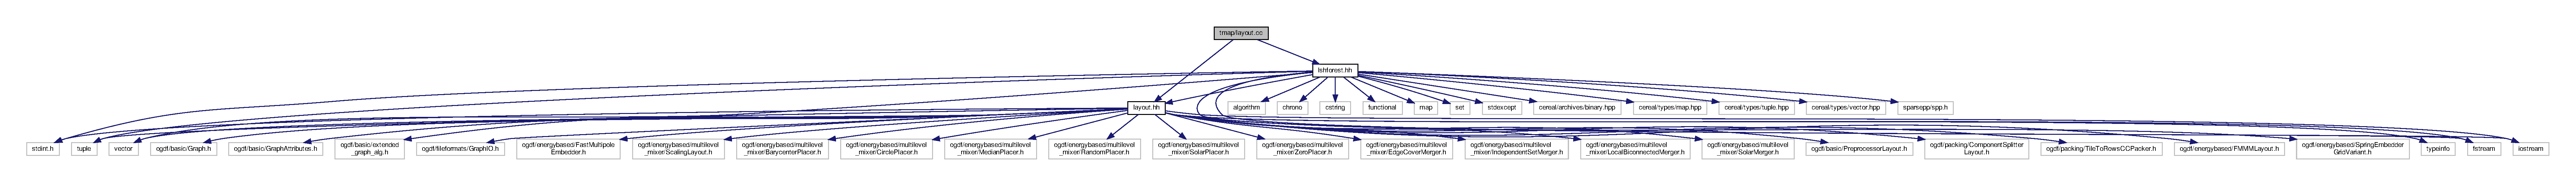
\includegraphics[width=350pt]{layout_8cc__incl}
\end{center}
\end{figure}
\subsection*{Functions}
\begin{DoxyCompactItemize}
\item 
\mbox{\Hypertarget{layout_8cc_a3d1a42c4bf2de56742f9ae91daf0bdec}\label{layout_8cc_a3d1a42c4bf2de56742f9ae91daf0bdec}} 
std\+::vector$<$ std\+::vector$<$ uint32\+\_\+t $>$ $>$ {\bfseries Get\+Trees\+From\+Forest} (const Graph \&g)
\item 
\mbox{\Hypertarget{layout_8cc_a9327106c87138ade0644c996cfa3a631}\label{layout_8cc_a9327106c87138ade0644c996cfa3a631}} 
void {\bfseries Remove\+Disconnected\+Components} (Graph \&g)
\item 
\mbox{\Hypertarget{layout_8cc_a4c768b7dc8cfc07697d2c470150c3574}\label{layout_8cc_a4c768b7dc8cfc07697d2c470150c3574}} 
void {\bfseries Connect\+Graph} (Graph \&g, std\+::vector$<$ node $>$ \&index\+\_\+to\+\_\+node, \hyperlink{classLSHForest}{L\+S\+H\+Forest} \&lsh\+\_\+forest)
\item 
std\+::tuple$<$ std\+::vector$<$ uint32\+\_\+t $>$, std\+::vector$<$ uint32\+\_\+t $>$ $>$ \hyperlink{layout_8cc_ad5464d8b1c40e92003702f14a5c4bf16}{M\+S\+T\+From\+L\+S\+H\+Forest} (\hyperlink{classLSHForest}{L\+S\+H\+Forest} \&lsh\+\_\+forest, uint32\+\_\+t k, uint32\+\_\+t kc, bool weighted)
\begin{DoxyCompactList}\small\item\em Generates an M\+ST (via a k\+NN graph) from an \hyperlink{classLSHForest}{L\+S\+H\+Forest} instance. \end{DoxyCompactList}\item 
std\+::tuple$<$ std\+::vector$<$ float $>$, std\+::vector$<$ float $>$, std\+::vector$<$ uint32\+\_\+t $>$, std\+::vector$<$ uint32\+\_\+t $>$, \hyperlink{structGraphProperties}{Graph\+Properties} $>$ \hyperlink{layout_8cc_a25c09eab65bee493ebb96ca9a001a12a}{Layout\+From\+L\+S\+H\+Forest} (\hyperlink{classLSHForest}{L\+S\+H\+Forest} \&lsh\+\_\+forest, \hyperlink{structLayoutConfiguration}{Layout\+Configuration} config, bool create\+\_\+mst, bool clear\+\_\+lsh\+\_\+forest, bool weighted)
\begin{DoxyCompactList}\small\item\em Genereates coordinates, edges and properties of a M\+ST (via a k\+NN graph) from an \hyperlink{classLSHForest}{L\+S\+H\+Forest} instance. \end{DoxyCompactList}\item 
std\+::tuple$<$ std\+::vector$<$ float $>$, std\+::vector$<$ float $>$, std\+::vector$<$ uint32\+\_\+t $>$, std\+::vector$<$ uint32\+\_\+t $>$, \hyperlink{structGraphProperties}{Graph\+Properties} $>$ \hyperlink{layout_8cc_a40835d0150427fd0f698c0a56b89b078}{Layout\+From\+Edge\+List} (uint32\+\_\+t vertex\+\_\+count, const std\+::vector$<$ std\+::tuple$<$ uint32\+\_\+t, uint32\+\_\+t, float $>$$>$ \&edges, \hyperlink{structLayoutConfiguration}{Layout\+Configuration} config, bool create\+\_\+mst)
\begin{DoxyCompactList}\small\item\em Genereates coordinates, edges and properties of a M\+ST from an edge list. \end{DoxyCompactList}\item 
\mbox{\Hypertarget{layout_8cc_afab0cb8f4e6f2a366445e32df3dedd9d}\label{layout_8cc_afab0cb8f4e6f2a366445e32df3dedd9d}} 
std\+::tuple$<$ std\+::vector$<$ float $>$, std\+::vector$<$ float $>$, std\+::vector$<$ uint32\+\_\+t $>$, std\+::vector$<$ uint32\+\_\+t $>$, \hyperlink{structGraphProperties}{Graph\+Properties} $>$ {\bfseries Layout\+Internal} (Edge\+Weighted\+Graph$<$ float $>$ \&g, uint32\+\_\+t vertex\+\_\+count, \hyperlink{structLayoutConfiguration}{Layout\+Configuration} config, \hyperlink{structGraphProperties}{Graph\+Properties} \&gp)
\end{DoxyCompactItemize}


\subsection{Detailed Description}
Functions used for generating graph layouts from \hyperlink{classLSHForest}{L\+S\+H\+Forest} instances and edge lists. 

\begin{DoxyAuthor}{Author}
Daniel Probst (\href{mailto:daenuprobst@gmail.com}{\tt daenuprobst@gmail.\+com}) 
\end{DoxyAuthor}
\begin{DoxyVersion}{Version}
0.\+1 
\end{DoxyVersion}
\begin{DoxyDate}{Date}
2019-\/06-\/17 
\end{DoxyDate}


\subsection{Function Documentation}
\mbox{\Hypertarget{layout_8cc_a40835d0150427fd0f698c0a56b89b078}\label{layout_8cc_a40835d0150427fd0f698c0a56b89b078}} 
\index{layout.\+cc@{layout.\+cc}!Layout\+From\+Edge\+List@{Layout\+From\+Edge\+List}}
\index{Layout\+From\+Edge\+List@{Layout\+From\+Edge\+List}!layout.\+cc@{layout.\+cc}}
\subsubsection{\texorpdfstring{Layout\+From\+Edge\+List()}{LayoutFromEdgeList()}}
{\footnotesize\ttfamily std\+::tuple$<$std\+::vector$<$float$>$, std\+::vector$<$float$>$, std\+::vector$<$uint32\+\_\+t$>$, std\+::vector$<$uint32\+\_\+t$>$, \hyperlink{structGraphProperties}{Graph\+Properties}$>$ Layout\+From\+Edge\+List (\begin{DoxyParamCaption}\item[{uint32\+\_\+t}]{vertex\+\_\+count,  }\item[{const std\+::vector$<$ std\+::tuple$<$ uint32\+\_\+t, uint32\+\_\+t, float $>$$>$ \&}]{edges,  }\item[{\hyperlink{structLayoutConfiguration}{Layout\+Configuration}}]{config = {\ttfamily \hyperlink{structLayoutConfiguration}{Layout\+Configuration}()},  }\item[{bool}]{create\+\_\+mst = {\ttfamily true} }\end{DoxyParamCaption})}



Genereates coordinates, edges and properties of a M\+ST from an edge list. 


\begin{DoxyParams}{Parameters}
{\em vertex\+\_\+count} & The number of vertices in the input graph. \\
\hline
{\em edges} & An edge list in the form of \mbox{[}(from, to, weight)\mbox{]}. \\
\hline
{\em config} & A \hyperlink{structLayoutConfiguration}{Layout\+Configuration} instance. \\
\hline
{\em create\+\_\+mst} & Whether to create an M\+ST before laying out the graph. \\
\hline
\end{DoxyParams}
\begin{DoxyReturn}{Returns}
std\+::tuple$<$std\+::vector$<$float$>$, std\+::vector$<$float$>$, std\+::vector$<$uint32\+\_\+t$>$, std\+::vector$<$uint32\+\_\+t$>$, \hyperlink{structGraphProperties}{Graph\+Properties}$>$ 
\end{DoxyReturn}
\mbox{\Hypertarget{layout_8cc_a25c09eab65bee493ebb96ca9a001a12a}\label{layout_8cc_a25c09eab65bee493ebb96ca9a001a12a}} 
\index{layout.\+cc@{layout.\+cc}!Layout\+From\+L\+S\+H\+Forest@{Layout\+From\+L\+S\+H\+Forest}}
\index{Layout\+From\+L\+S\+H\+Forest@{Layout\+From\+L\+S\+H\+Forest}!layout.\+cc@{layout.\+cc}}
\subsubsection{\texorpdfstring{Layout\+From\+L\+S\+H\+Forest()}{LayoutFromLSHForest()}}
{\footnotesize\ttfamily std\+::tuple$<$std\+::vector$<$float$>$, std\+::vector$<$float$>$, std\+::vector$<$uint32\+\_\+t$>$, std\+::vector$<$uint32\+\_\+t$>$, \hyperlink{structGraphProperties}{Graph\+Properties}$>$ Layout\+From\+L\+S\+H\+Forest (\begin{DoxyParamCaption}\item[{\hyperlink{classLSHForest}{L\+S\+H\+Forest} \&}]{lsh\+\_\+forest,  }\item[{\hyperlink{structLayoutConfiguration}{Layout\+Configuration}}]{config = {\ttfamily \hyperlink{structLayoutConfiguration}{Layout\+Configuration}()},  }\item[{bool}]{create\+\_\+mst = {\ttfamily true},  }\item[{bool}]{clear\+\_\+lsh\+\_\+forest = {\ttfamily false},  }\item[{bool}]{weighted = {\ttfamily false} }\end{DoxyParamCaption})}



Genereates coordinates, edges and properties of a M\+ST (via a k\+NN graph) from an \hyperlink{classLSHForest}{L\+S\+H\+Forest} instance. 


\begin{DoxyParams}{Parameters}
{\em lsh\+\_\+forest} & An \hyperlink{classLSHForest}{L\+S\+H\+Forest} instance which is used to construct the k\+NN graph. \\
\hline
{\em config} & A \hyperlink{structLayoutConfiguration}{Layout\+Configuration} instance. \\
\hline
{\em create\+\_\+mst} & Whether to create an M\+ST before laying out the graph. \\
\hline
{\em clear\+\_\+lsh\+\_\+forest} & Whether to clear the \hyperlink{classLSHForest}{L\+S\+H\+Forest} after it\textquotesingle{}s use (might save memory). \\
\hline
{\em weighted} & Whether the \hyperlink{classLSHForest}{L\+S\+H\+Forest} instance contains weighted Min\+Hash data. \\
\hline
\end{DoxyParams}
\begin{DoxyReturn}{Returns}
std\+::tuple$<$std\+::vector$<$float$>$, std\+::vector$<$float$>$, std\+::vector$<$uint32\+\_\+t$>$, std\+::vector$<$uint32\+\_\+t$>$, \hyperlink{structGraphProperties}{Graph\+Properties}$>$ 
\end{DoxyReturn}
\mbox{\Hypertarget{layout_8cc_ad5464d8b1c40e92003702f14a5c4bf16}\label{layout_8cc_ad5464d8b1c40e92003702f14a5c4bf16}} 
\index{layout.\+cc@{layout.\+cc}!M\+S\+T\+From\+L\+S\+H\+Forest@{M\+S\+T\+From\+L\+S\+H\+Forest}}
\index{M\+S\+T\+From\+L\+S\+H\+Forest@{M\+S\+T\+From\+L\+S\+H\+Forest}!layout.\+cc@{layout.\+cc}}
\subsubsection{\texorpdfstring{M\+S\+T\+From\+L\+S\+H\+Forest()}{MSTFromLSHForest()}}
{\footnotesize\ttfamily std\+::tuple$<$std\+::vector$<$uint32\+\_\+t$>$, std\+::vector$<$uint32\+\_\+t$>$ $>$ M\+S\+T\+From\+L\+S\+H\+Forest (\begin{DoxyParamCaption}\item[{\hyperlink{classLSHForest}{L\+S\+H\+Forest} \&}]{lsh\+\_\+forest,  }\item[{uint32\+\_\+t}]{k,  }\item[{uint32\+\_\+t}]{kc = {\ttfamily 10},  }\item[{bool}]{weighted = {\ttfamily false} }\end{DoxyParamCaption})}



Generates an M\+ST (via a k\+NN graph) from an \hyperlink{classLSHForest}{L\+S\+H\+Forest} instance. 


\begin{DoxyParams}{Parameters}
{\em lsh\+\_\+forest} & An \hyperlink{classLSHForest}{L\+S\+H\+Forest} instance which is used to construct the k\+NN graph. \\
\hline
{\em k} & The number of nearest neighbors used to create the k\+NN graph. \\
\hline
{\em kc} & The factor by which k is multiplied when retrieving nearest neighbors. \\
\hline
{\em weighted} & Whether the \hyperlink{classLSHForest}{L\+S\+H\+Forest} instance contains weighted Min\+Hash data. \\
\hline
\end{DoxyParams}
\begin{DoxyReturn}{Returns}
std\+::tuple$<$std\+::vector$<$uint32\+\_\+t$>$, std\+::vector$<$uint32\+\_\+t$>$$>$ 
\end{DoxyReturn}

\hypertarget{layout_8hh}{}\section{src/tmap/layout.hh File Reference}
\label{layout_8hh}\index{src/tmap/layout.\+hh@{src/tmap/layout.\+hh}}


Functions used for generating graph layouts from L\+S\+H\+Forest instances and edge lists.  


{\ttfamily \#include $<$vector$>$}\newline
{\ttfamily \#include $<$tuple$>$}\newline
{\ttfamily \#include $<$stdint.\+h$>$}\newline
{\ttfamily \#include $<$ogdf/basic/\+Graph.\+h$>$}\newline
{\ttfamily \#include $<$ogdf/fileformats/\+Graph\+I\+O.\+h$>$}\newline
{\ttfamily \#include $<$ogdf/basic/\+Graph\+Attributes.\+h$>$}\newline
{\ttfamily \#include $<$ogdf/basic/extended\+\_\+graph\+\_\+alg.\+h$>$}\newline
{\ttfamily \#include $<$ogdf/energybased/\+Fast\+Multipole\+Embedder.\+h$>$}\newline
{\ttfamily \#include $<$ogdf/energybased/multilevel\+\_\+mixer/\+Scaling\+Layout.\+h$>$}\newline
{\ttfamily \#include $<$ogdf/energybased/multilevel\+\_\+mixer/\+Barycenter\+Placer.\+h$>$}\newline
{\ttfamily \#include $<$ogdf/energybased/multilevel\+\_\+mixer/\+Solar\+Placer.\+h$>$}\newline
{\ttfamily \#include $<$ogdf/energybased/multilevel\+\_\+mixer/\+Circle\+Placer.\+h$>$}\newline
{\ttfamily \#include $<$ogdf/energybased/multilevel\+\_\+mixer/\+Median\+Placer.\+h$>$}\newline
{\ttfamily \#include $<$ogdf/energybased/multilevel\+\_\+mixer/\+Random\+Placer.\+h$>$}\newline
{\ttfamily \#include $<$ogdf/energybased/multilevel\+\_\+mixer/\+Zero\+Placer.\+h$>$}\newline
{\ttfamily \#include $<$ogdf/energybased/multilevel\+\_\+mixer/\+Solar\+Merger.\+h$>$}\newline
{\ttfamily \#include $<$ogdf/energybased/multilevel\+\_\+mixer/\+Edge\+Cover\+Merger.\+h$>$}\newline
{\ttfamily \#include $<$ogdf/energybased/multilevel\+\_\+mixer/\+Independent\+Set\+Merger.\+h$>$}\newline
{\ttfamily \#include $<$ogdf/energybased/multilevel\+\_\+mixer/\+Local\+Biconnected\+Merger.\+h$>$}\newline
{\ttfamily \#include $<$ogdf/basic/\+Preprocessor\+Layout.\+h$>$}\newline
{\ttfamily \#include $<$ogdf/packing/\+Component\+Splitter\+Layout.\+h$>$}\newline
{\ttfamily \#include $<$ogdf/packing/\+Tile\+To\+Rows\+C\+C\+Packer.\+h$>$}\newline
{\ttfamily \#include $<$ogdf/energybased/\+F\+M\+M\+M\+Layout.\+h$>$}\newline
{\ttfamily \#include $<$ogdf/energybased/\+Spring\+Embedder\+Grid\+Variant.\+h$>$}\newline
{\ttfamily \#include $<$iostream$>$}\newline
{\ttfamily \#include $<$fstream$>$}\newline
{\ttfamily \#include $<$typeinfo$>$}\newline
Include dependency graph for layout.\+hh\+:\nopagebreak
\begin{figure}[H]
\begin{center}
\leavevmode
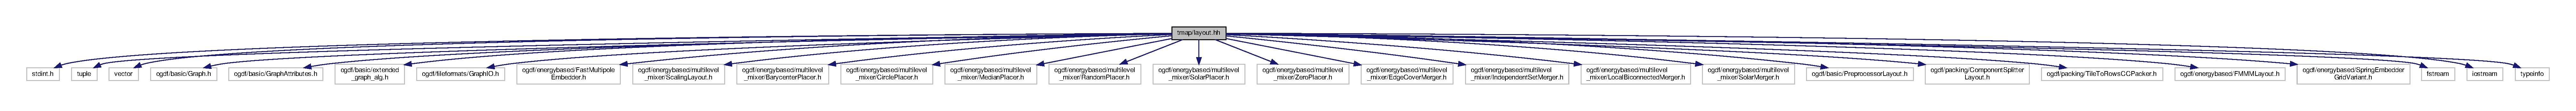
\includegraphics[width=350pt]{layout_8hh__incl}
\end{center}
\end{figure}
This graph shows which files directly or indirectly include this file\+:\nopagebreak
\begin{figure}[H]
\begin{center}
\leavevmode
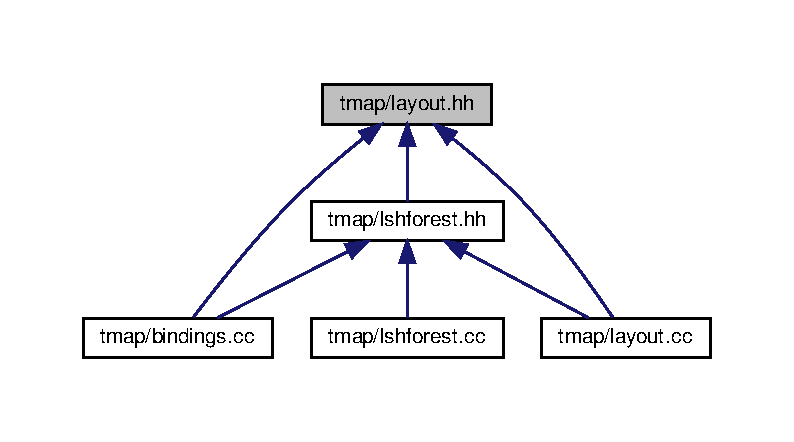
\includegraphics[width=350pt]{layout_8hh__dep__incl}
\end{center}
\end{figure}
\subsection*{Classes}
\begin{DoxyCompactItemize}
\item 
struct \hyperlink{structtmap_1_1LayoutConfiguration}{tmap\+::\+Layout\+Configuration}
\begin{DoxyCompactList}\small\item\em A struct containing all the configuration options available for and applied to a layout. \end{DoxyCompactList}\item 
struct \hyperlink{structtmap_1_1GraphProperties}{tmap\+::\+Graph\+Properties}
\begin{DoxyCompactList}\small\item\em The properties of a generated graph. An instance of this struct is returned from the layout functions. \end{DoxyCompactList}\end{DoxyCompactItemize}
\subsection*{Enumerations}
\begin{DoxyCompactItemize}
\item 
\mbox{\Hypertarget{layout_8hh_afdc98947e81dc6f4c30f256e6f42f90b}\label{layout_8hh_afdc98947e81dc6f4c30f256e6f42f90b}} 
enum \hyperlink{layout_8hh_afdc98947e81dc6f4c30f256e6f42f90b}{tmap\+::\+Placer} \{ \newline
{\bfseries tmap\+::\+Placer\+::\+Barycenter} = 0, 
{\bfseries tmap\+::\+Placer\+::\+Solar} = 1, 
{\bfseries tmap\+::\+Placer\+::\+Circle} = 2, 
{\bfseries tmap\+::\+Placer\+::\+Median} = 3, 
\newline
{\bfseries tmap\+::\+Placer\+::\+Random} = 4, 
{\bfseries tmap\+::\+Placer\+::\+Zero} = 5
 \}\begin{DoxyCompactList}\small\item\em The placers available in O\+G\+DF. \end{DoxyCompactList}
\item 
\mbox{\Hypertarget{layout_8hh_a8c7bb9956a1a724233182a166cfdc0ff}\label{layout_8hh_a8c7bb9956a1a724233182a166cfdc0ff}} 
enum \hyperlink{layout_8hh_a8c7bb9956a1a724233182a166cfdc0ff}{tmap\+::\+Merger} \{ {\bfseries tmap\+::\+Merger\+::\+Edge\+Cover} = 0, 
{\bfseries tmap\+::\+Merger\+::\+Local\+Biconnected} = 1, 
{\bfseries tmap\+::\+Merger\+::\+Solar} = 2, 
{\bfseries tmap\+::\+Merger\+::\+Independent\+Set} = 3
 \}\begin{DoxyCompactList}\small\item\em The mergers available in O\+G\+DF. \end{DoxyCompactList}
\item 
\mbox{\Hypertarget{layout_8hh_a50ec215c9e54cf12b9dd0a0056160761}\label{layout_8hh_a50ec215c9e54cf12b9dd0a0056160761}} 
enum \hyperlink{layout_8hh_a50ec215c9e54cf12b9dd0a0056160761}{tmap\+::\+Scaling\+Type} \{ {\bfseries tmap\+::\+Scaling\+Type\+::\+Absolute} = 0, 
{\bfseries tmap\+::\+Scaling\+Type\+::\+Relative\+To\+Avg\+Length} = 1, 
{\bfseries tmap\+::\+Scaling\+Type\+::\+Relative\+To\+Desired\+Length} = 2, 
{\bfseries tmap\+::\+Scaling\+Type\+::\+Relative\+To\+Drawing} = 3
 \}\begin{DoxyCompactList}\small\item\em The scaling types available in O\+G\+DF. \end{DoxyCompactList}
\end{DoxyCompactItemize}
\subsection*{Functions}
\begin{DoxyCompactItemize}
\item 
std\+::tuple$<$ std\+::vector$<$ float $>$, std\+::vector$<$ float $>$, std\+::vector$<$ uint32\+\_\+t $>$, std\+::vector$<$ uint32\+\_\+t $>$, Graph\+Properties $>$ \hyperlink{layout_8hh_acd9c409403d706202320359541674ba8}{tmap\+::\+Layout\+From\+L\+S\+H\+Forest} (L\+S\+H\+Forest \&lsh\+\_\+forest, Layout\+Configuration config=Layout\+Configuration(), bool create\+\_\+mst=true, bool clear\+\_\+lsh\+\_\+forest=false, bool weighted=false)
\begin{DoxyCompactList}\small\item\em Genereates coordinates, edges and properties of a M\+ST (via a k\+NN graph) from an \hyperlink{classtmap_1_1LSHForest}{L\+S\+H\+Forest} instance. \end{DoxyCompactList}\item 
std\+::tuple$<$ std\+::vector$<$ uint32\+\_\+t $>$, std\+::vector$<$ uint32\+\_\+t $>$ $>$ \hyperlink{layout_8hh_a3d7180c2fcc2a1ec72838f18177d6840}{tmap\+::\+M\+S\+T\+From\+L\+S\+H\+Forest} (L\+S\+H\+Forest \&lsh\+\_\+forest, uint32\+\_\+t k, uint32\+\_\+t kc=10, bool weighted=false)
\begin{DoxyCompactList}\small\item\em Generates an M\+ST (via a k\+NN graph) from an \hyperlink{classtmap_1_1LSHForest}{L\+S\+H\+Forest} instance. \end{DoxyCompactList}\item 
std\+::tuple$<$ std\+::vector$<$ float $>$, std\+::vector$<$ float $>$, std\+::vector$<$ uint32\+\_\+t $>$, std\+::vector$<$ uint32\+\_\+t $>$, Graph\+Properties $>$ \hyperlink{layout_8hh_a780993ad8dd7e349b77f55895cc33451}{tmap\+::\+Layout\+From\+Edge\+List} (uint32\+\_\+t vertex\+\_\+count, const std\+::vector$<$ std\+::tuple$<$ uint32\+\_\+t, uint32\+\_\+t, float $>$$>$ \&edges, Layout\+Configuration config=Layout\+Configuration(), bool create\+\_\+mst=true)
\begin{DoxyCompactList}\small\item\em Genereates coordinates, edges and properties of a M\+ST from an edge list. \end{DoxyCompactList}\item 
std\+::tuple$<$ std\+::vector$<$ float $>$, std\+::vector$<$ float $>$, std\+::vector$<$ uint32\+\_\+t $>$, std\+::vector$<$ uint32\+\_\+t $>$, Graph\+Properties $>$ \hyperlink{layout_8hh_a126dbc6ec8355732c528abb2877e60d4}{tmap\+::\+Layout\+Internal} (ogdf\+::\+Edge\+Weighted\+Graph$<$ float $>$ \&g, uint32\+\_\+t vertex\+\_\+count, Layout\+Configuration config, Graph\+Properties \&gp)
\begin{DoxyCompactList}\small\item\em Laying out an O\+G\+DF graph. \end{DoxyCompactList}\end{DoxyCompactItemize}


\subsection{Detailed Description}
Functions used for generating graph layouts from L\+S\+H\+Forest instances and edge lists. 

\begin{DoxyAuthor}{Author}
Daniel Probst (\href{mailto:daenuprobst@gmail.com}{\tt daenuprobst@gmail.\+com}) 
\end{DoxyAuthor}
\begin{DoxyVersion}{Version}
0.\+1 
\end{DoxyVersion}
\begin{DoxyDate}{Date}
2019-\/06-\/17 
\end{DoxyDate}


\subsection{Function Documentation}
\mbox{\Hypertarget{layout_8hh_file_a780993ad8dd7e349b77f55895cc33451}\label{layout_8hh_file_a780993ad8dd7e349b77f55895cc33451}} 
\index{layout.\+hh@{layout.\+hh}!Layout\+From\+Edge\+List@{Layout\+From\+Edge\+List}}
\index{Layout\+From\+Edge\+List@{Layout\+From\+Edge\+List}!layout.\+hh@{layout.\+hh}}
\subsubsection{\texorpdfstring{Layout\+From\+Edge\+List()}{LayoutFromEdgeList()}}
{\footnotesize\ttfamily std\+::tuple$<$ std\+::vector$<$ float $>$, std\+::vector$<$ float $>$, std\+::vector$<$ uint32\+\_\+t $>$, std\+::vector$<$ uint32\+\_\+t $>$, \hyperlink{structtmap_1_1GraphProperties}{tmap\+::\+Graph\+Properties} $>$ tmap\+::\+Layout\+From\+Edge\+List (\begin{DoxyParamCaption}\item[{uint32\+\_\+t}]{vertex\+\_\+count,  }\item[{const std\+::vector$<$ std\+::tuple$<$ uint32\+\_\+t, uint32\+\_\+t, float $>$$>$ \&}]{edges,  }\item[{\hyperlink{structtmap_1_1LayoutConfiguration}{tmap\+::\+Layout\+Configuration}}]{config = {\ttfamily \hyperlink{structtmap_1_1LayoutConfiguration}{Layout\+Configuration}()},  }\item[{bool}]{create\+\_\+mst = {\ttfamily true} }\end{DoxyParamCaption})}



Genereates coordinates, edges and properties of a M\+ST from an edge list. 


\begin{DoxyParams}{Parameters}
{\em vertex\+\_\+count} & The number of vertices in the input graph. \\
\hline
{\em edges} & An edge list in the form of \mbox{[}(from, to, weight)\mbox{]}. \\
\hline
{\em config} & A Layout\+Configuration instance. \\
\hline
{\em create\+\_\+mst} & Whether to create an M\+ST before laying out the graph. \\
\hline
\end{DoxyParams}
\begin{DoxyReturn}{Returns}
std\+::tuple$<$std\+::vector$<$float$>$, std\+::vector$<$float$>$, std\+::vector$<$uint32\+\_\+t$>$, std\+::vector$<$uint32\+\_\+t$>$, Graph\+Properties$>$ 
\end{DoxyReturn}
\mbox{\Hypertarget{layout_8hh_file_acd9c409403d706202320359541674ba8}\label{layout_8hh_file_acd9c409403d706202320359541674ba8}} 
\index{layout.\+hh@{layout.\+hh}!Layout\+From\+L\+S\+H\+Forest@{Layout\+From\+L\+S\+H\+Forest}}
\index{Layout\+From\+L\+S\+H\+Forest@{Layout\+From\+L\+S\+H\+Forest}!layout.\+hh@{layout.\+hh}}
\subsubsection{\texorpdfstring{Layout\+From\+L\+S\+H\+Forest()}{LayoutFromLSHForest()}}
{\footnotesize\ttfamily std\+::tuple$<$ std\+::vector$<$ float $>$, std\+::vector$<$ float $>$, std\+::vector$<$ uint32\+\_\+t $>$, std\+::vector$<$ uint32\+\_\+t $>$, \hyperlink{structtmap_1_1GraphProperties}{tmap\+::\+Graph\+Properties} $>$ tmap\+::\+Layout\+From\+L\+S\+H\+Forest (\begin{DoxyParamCaption}\item[{\hyperlink{classtmap_1_1LSHForest}{tmap\+::\+L\+S\+H\+Forest} \&}]{lsh\+\_\+forest,  }\item[{\hyperlink{structtmap_1_1LayoutConfiguration}{tmap\+::\+Layout\+Configuration}}]{config = {\ttfamily \hyperlink{structtmap_1_1LayoutConfiguration}{Layout\+Configuration}()},  }\item[{bool}]{create\+\_\+mst = {\ttfamily true},  }\item[{bool}]{clear\+\_\+lsh\+\_\+forest = {\ttfamily false},  }\item[{bool}]{weighted = {\ttfamily false} }\end{DoxyParamCaption})}



Genereates coordinates, edges and properties of a M\+ST (via a k\+NN graph) from an L\+S\+H\+Forest instance. 


\begin{DoxyParams}{Parameters}
{\em lsh\+\_\+forest} & An L\+S\+H\+Forest instance which is used to construct the k\+NN graph. \\
\hline
{\em config} & A Layout\+Configuration instance. \\
\hline
{\em create\+\_\+mst} & Whether to create an M\+ST before laying out the graph. \\
\hline
{\em clear\+\_\+lsh\+\_\+forest} & Whether to clear the L\+S\+H\+Forest after it\textquotesingle{}s use (might save memory). \\
\hline
{\em weighted} & Whether the L\+S\+H\+Forest instance contains weighted Min\+Hash data. \\
\hline
\end{DoxyParams}
\begin{DoxyReturn}{Returns}
std\+::tuple$<$std\+::vector$<$float$>$, std\+::vector$<$float$>$, std\+::vector$<$uint32\+\_\+t$>$, std\+::vector$<$uint32\+\_\+t$>$, Graph\+Properties$>$ 
\end{DoxyReturn}
\mbox{\Hypertarget{layout_8hh_file_a126dbc6ec8355732c528abb2877e60d4}\label{layout_8hh_file_a126dbc6ec8355732c528abb2877e60d4}} 
\index{layout.\+hh@{layout.\+hh}!Layout\+Internal@{Layout\+Internal}}
\index{Layout\+Internal@{Layout\+Internal}!layout.\+hh@{layout.\+hh}}
\subsubsection{\texorpdfstring{Layout\+Internal()}{LayoutInternal()}}
{\footnotesize\ttfamily std\+::tuple$<$std\+::vector$<$float$>$, std\+::vector$<$float$>$, std\+::vector$<$uint32\+\_\+t$>$, std\+::vector$<$uint32\+\_\+t$>$, Graph\+Properties$>$ tmap\+::\+Layout\+Internal (\begin{DoxyParamCaption}\item[{ogdf\+::\+Edge\+Weighted\+Graph$<$ float $>$ \&}]{g,  }\item[{uint32\+\_\+t}]{vertex\+\_\+count,  }\item[{\hyperlink{structtmap_1_1LayoutConfiguration}{Layout\+Configuration}}]{config,  }\item[{\hyperlink{structtmap_1_1GraphProperties}{Graph\+Properties} \&}]{gp }\end{DoxyParamCaption})}



Laying out an O\+G\+DF graph. 


\begin{DoxyParams}{Parameters}
{\em g} & An O\+G\+DF Graph instance \\
\hline
{\em vertex\+\_\+count} & The number of vertices in the graph. \\
\hline
{\em config} & A Layout\+Configuration instance. \\
\hline
{\em gp} & An instance of a Graph\+Properties struct. \\
\hline
\end{DoxyParams}
\begin{DoxyReturn}{Returns}
std\+::tuple$<$std\+::vector$<$float$>$, std\+::vector$<$float$>$, std\+::vector$<$uint32\+\_\+t$>$, std\+::vector$<$uint32\+\_\+t$>$, Graph\+Properties$>$ 
\end{DoxyReturn}
\mbox{\Hypertarget{layout_8hh_file_a3d7180c2fcc2a1ec72838f18177d6840}\label{layout_8hh_file_a3d7180c2fcc2a1ec72838f18177d6840}} 
\index{layout.\+hh@{layout.\+hh}!M\+S\+T\+From\+L\+S\+H\+Forest@{M\+S\+T\+From\+L\+S\+H\+Forest}}
\index{M\+S\+T\+From\+L\+S\+H\+Forest@{M\+S\+T\+From\+L\+S\+H\+Forest}!layout.\+hh@{layout.\+hh}}
\subsubsection{\texorpdfstring{M\+S\+T\+From\+L\+S\+H\+Forest()}{MSTFromLSHForest()}}
{\footnotesize\ttfamily std\+::tuple$<$ std\+::vector$<$ uint32\+\_\+t $>$, std\+::vector$<$ uint32\+\_\+t $>$ $>$ tmap\+::\+M\+S\+T\+From\+L\+S\+H\+Forest (\begin{DoxyParamCaption}\item[{\hyperlink{classtmap_1_1LSHForest}{tmap\+::\+L\+S\+H\+Forest} \&}]{lsh\+\_\+forest,  }\item[{uint32\+\_\+t}]{k,  }\item[{uint32\+\_\+t}]{kc = {\ttfamily 10},  }\item[{bool}]{weighted = {\ttfamily false} }\end{DoxyParamCaption})}



Generates an M\+ST (via a k\+NN graph) from an L\+S\+H\+Forest instance. 


\begin{DoxyParams}{Parameters}
{\em lsh\+\_\+forest} & An L\+S\+H\+Forest instance which is used to construct the k\+NN graph. \\
\hline
{\em k} & The number of nearest neighbors used to create the k\+NN graph. \\
\hline
{\em kc} & The factor by which k is multiplied when retrieving nearest neighbors. \\
\hline
{\em weighted} & Whether the L\+S\+H\+Forest instance contains weighted Min\+Hash data. \\
\hline
\end{DoxyParams}
\begin{DoxyReturn}{Returns}
std\+::tuple$<$std\+::vector$<$uint32\+\_\+t$>$, std\+::vector$<$uint32\+\_\+t$>$$>$ 
\end{DoxyReturn}

\hypertarget{lshforest_8cc}{}\section{tmap/lshforest.cc File Reference}
\label{lshforest_8cc}\index{tmap/lshforest.\+cc@{tmap/lshforest.\+cc}}


An L\+SH forest algorithm implementation.  


{\ttfamily \#include \char`\"{}lshforest.\+hh\char`\"{}}\newline
Include dependency graph for lshforest.\+cc\+:\nopagebreak
\begin{figure}[H]
\begin{center}
\leavevmode
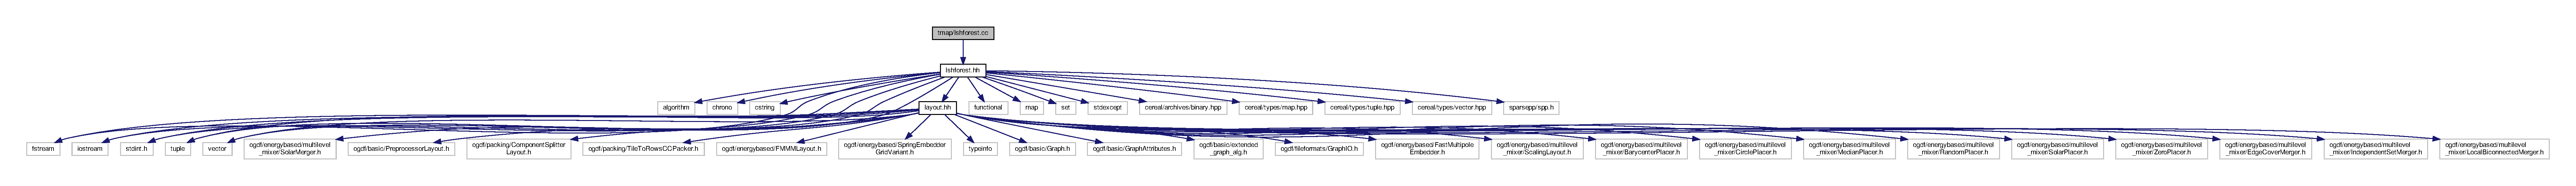
\includegraphics[width=350pt]{lshforest_8cc__incl}
\end{center}
\end{figure}


\subsection{Detailed Description}
An L\+SH forest algorithm implementation. 

\begin{DoxyAuthor}{Author}
Daniel Probst (\href{mailto:daenuprobst@gmail.com}{\tt daenuprobst@gmail.\+com}) 
\end{DoxyAuthor}
\begin{DoxyVersion}{Version}
0.\+1 
\end{DoxyVersion}
\begin{DoxyDate}{Date}
2019-\/06-\/17 
\end{DoxyDate}

\hypertarget{lshforest_8hh}{}\section{tmap/lshforest.hh File Reference}
\label{lshforest_8hh}\index{tmap/lshforest.\+hh@{tmap/lshforest.\+hh}}


An L\+SH forest algorithm implementation.  


{\ttfamily \#include $<$algorithm$>$}\newline
{\ttfamily \#include $<$chrono$>$}\newline
{\ttfamily \#include $<$cstring$>$}\newline
{\ttfamily \#include $<$fstream$>$}\newline
{\ttfamily \#include $<$functional$>$}\newline
{\ttfamily \#include $<$iostream$>$}\newline
{\ttfamily \#include $<$map$>$}\newline
{\ttfamily \#include $<$set$>$}\newline
{\ttfamily \#include $<$stdexcept$>$}\newline
{\ttfamily \#include $<$stdint.\+h$>$}\newline
{\ttfamily \#include $<$tuple$>$}\newline
{\ttfamily \#include $<$vector$>$}\newline
{\ttfamily \#include \char`\"{}cereal/archives/binary.\+hpp\char`\"{}}\newline
{\ttfamily \#include \char`\"{}cereal/types/map.\+hpp\char`\"{}}\newline
{\ttfamily \#include \char`\"{}cereal/types/tuple.\+hpp\char`\"{}}\newline
{\ttfamily \#include \char`\"{}cereal/types/vector.\+hpp\char`\"{}}\newline
{\ttfamily \#include \char`\"{}layout.\+hh\char`\"{}}\newline
{\ttfamily \#include \char`\"{}sparsepp/spp.\+h\char`\"{}}\newline
Include dependency graph for lshforest.\+hh\+:\nopagebreak
\begin{figure}[H]
\begin{center}
\leavevmode
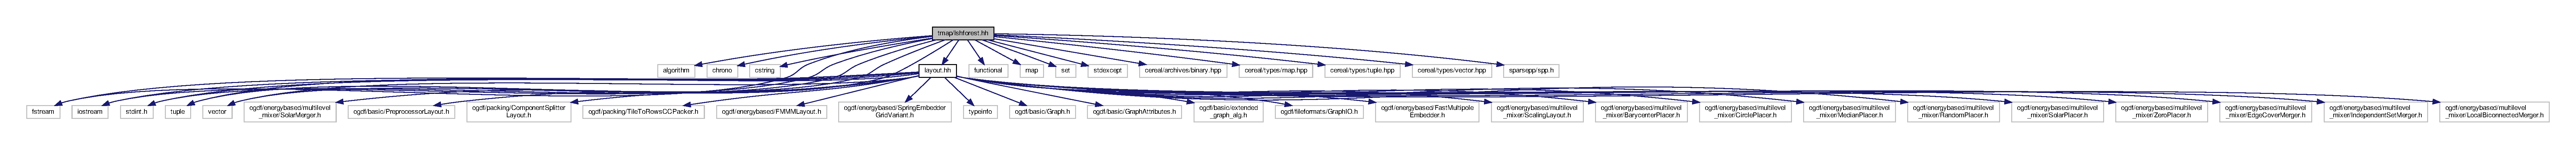
\includegraphics[width=350pt]{lshforest_8hh__incl}
\end{center}
\end{figure}
This graph shows which files directly or indirectly include this file\+:\nopagebreak
\begin{figure}[H]
\begin{center}
\leavevmode
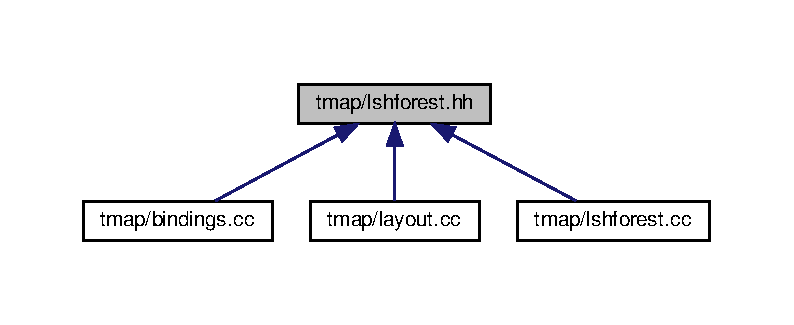
\includegraphics[width=350pt]{lshforest_8hh__dep__incl}
\end{center}
\end{figure}
\subsection*{Classes}
\begin{DoxyCompactItemize}
\item 
struct \hyperlink{structtmap_1_1SimpleHash}{tmap\+::\+Simple\+Hash}
\begin{DoxyCompactList}\small\item\em Hash struct used for the sparsepp sparse hash map. \end{DoxyCompactList}\item 
struct \hyperlink{structtmap_1_1MapKeyPointer}{tmap\+::\+Map\+Key\+Pointer}
\begin{DoxyCompactList}\small\item\em The pointer map used for pointing to the keys from the sorted hash map. \end{DoxyCompactList}\item 
class \hyperlink{classtmap_1_1Timer}{tmap\+::\+Timer}
\begin{DoxyCompactList}\small\item\em A simple timer class used to check performance during development. \end{DoxyCompactList}\item 
class \hyperlink{classtmap_1_1LSHForest}{tmap\+::\+L\+S\+H\+Forest}
\begin{DoxyCompactList}\small\item\em Provides locality sensitive hashing forest functionalities. \end{DoxyCompactList}\end{DoxyCompactItemize}


\subsection{Detailed Description}
An L\+SH forest algorithm implementation. 

\begin{DoxyAuthor}{Author}
Daniel Probst (\href{mailto:daenuprobst@gmail.com}{\tt daenuprobst@gmail.\+com}) 
\end{DoxyAuthor}
\begin{DoxyVersion}{Version}
0.\+1 
\end{DoxyVersion}
\begin{DoxyDate}{Date}
2019-\/06-\/17 
\end{DoxyDate}

\hypertarget{minhash_8cc}{}\section{tmap/minhash.cc File Reference}
\label{minhash_8cc}\index{tmap/minhash.\+cc@{tmap/minhash.\+cc}}


A Min\+Hash algorithm implementation.  


{\ttfamily \#include \char`\"{}minhash.\+hh\char`\"{}}\newline
Include dependency graph for minhash.\+cc\+:\nopagebreak
\begin{figure}[H]
\begin{center}
\leavevmode
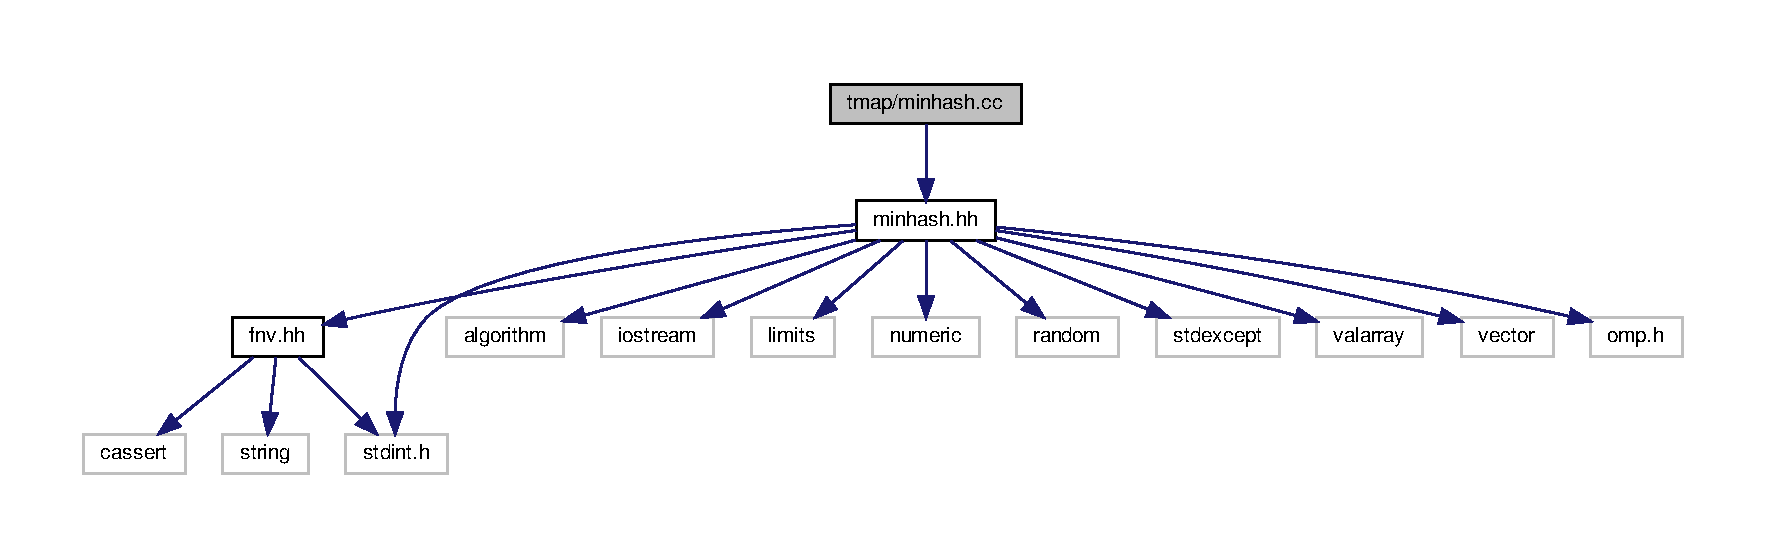
\includegraphics[width=350pt]{minhash_8cc__incl}
\end{center}
\end{figure}


\subsection{Detailed Description}
A Min\+Hash algorithm implementation. 

\begin{DoxyAuthor}{Author}
Daniel Probst (\href{mailto:daenuprobst@gmail.com}{\tt daenuprobst@gmail.\+com}) 
\end{DoxyAuthor}
\begin{DoxyVersion}{Version}
0.\+1 
\end{DoxyVersion}
\begin{DoxyDate}{Date}
2019-\/06-\/17 
\end{DoxyDate}

\hypertarget{minhash_8hh}{}\section{tmap/minhash.hh File Reference}
\label{minhash_8hh}\index{tmap/minhash.\+hh@{tmap/minhash.\+hh}}


A Min\+Hash algorithm implementation.  


{\ttfamily \#include \char`\"{}fnv.\+hh\char`\"{}}\newline
{\ttfamily \#include $<$algorithm$>$}\newline
{\ttfamily \#include $<$iostream$>$}\newline
{\ttfamily \#include $<$limits$>$}\newline
{\ttfamily \#include $<$numeric$>$}\newline
{\ttfamily \#include $<$random$>$}\newline
{\ttfamily \#include $<$stdexcept$>$}\newline
{\ttfamily \#include $<$stdint.\+h$>$}\newline
{\ttfamily \#include $<$math.\+h$>$}\newline
{\ttfamily \#include $<$vector$>$}\newline
{\ttfamily \#include \char`\"{}omp.\+h\char`\"{}}\newline
Include dependency graph for minhash.\+hh\+:\nopagebreak
\begin{figure}[H]
\begin{center}
\leavevmode
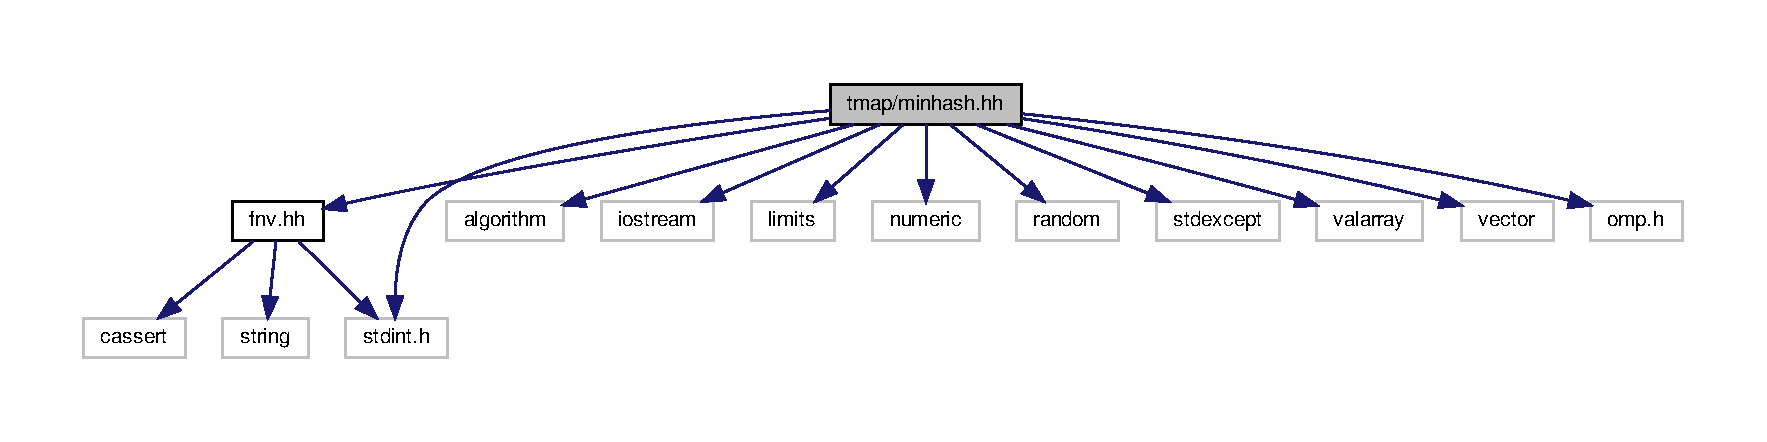
\includegraphics[width=350pt]{minhash_8hh__incl}
\end{center}
\end{figure}
This graph shows which files directly or indirectly include this file\+:\nopagebreak
\begin{figure}[H]
\begin{center}
\leavevmode
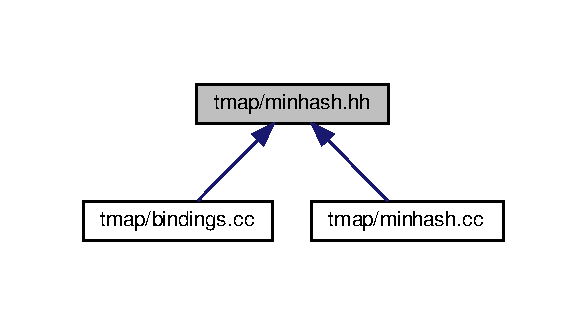
\includegraphics[width=282pt]{minhash_8hh__dep__incl}
\end{center}
\end{figure}
\subsection*{Classes}
\begin{DoxyCompactItemize}
\item 
class \hyperlink{classtmap_1_1Minhash}{tmap\+::\+Minhash}
\begin{DoxyCompactList}\small\item\em An implementation of Min\+Hash and weighted Min\+Hash using S\+H\+A1. \end{DoxyCompactList}\end{DoxyCompactItemize}


\subsection{Detailed Description}
A Min\+Hash algorithm implementation. 

\begin{DoxyAuthor}{Author}
Daniel Probst (\href{mailto:daenuprobst@gmail.com}{\tt daenuprobst@gmail.\+com}) 
\end{DoxyAuthor}
\begin{DoxyVersion}{Version}
0.\+1 
\end{DoxyVersion}
\begin{DoxyDate}{Date}
2019-\/06-\/17 
\end{DoxyDate}

%--- End generated contents ---

% Index
\backmatter
\newpage
\phantomsection
\clearemptydoublepage
\addcontentsline{toc}{chapter}{Index}
\printindex

\end{document}
